
\documentclass[12pt]{article}
\usepackage[UTF8]{ctex}

% Set page size and margins

\usepackage[a4paper,top=2cm,bottom=2cm,left=2cm,right=2cm,marginparwidth=1.75cm]{geometry}
\usepackage[ruled]{algorithm2e}
%\usepackage[hidelinks,colorlinks = true, allcolors = blue]{hyperref}
\usepackage{amsmath}
\usepackage{caption}
\usepackage{booktabs}
\usepackage{subfig}
\usepackage{graphicx}
\usepackage{makecell}
\usepackage{amsmath}
\usepackage{hyperref}
% 格式设置
\hypersetup{hidelinks,
	colorlinks=true,
	allcolors=black,
	pdfstartview=Fit,
	breaklinks=true}
\usepackage{listings}
\renewcommand{\thefigure}{\thesection{}-\arabic{figure}}
\lstset{
    basicstyle          =   \sffamily,          % 基本代码风格
    keywordstyle        =   \bfseries,          % 关键字风格
    commentstyle        =   \rmfamily\itshape,  % 注释的风格,斜体
    stringstyle         =   \ttfamily,  % 字符串风格
    flexiblecolumns,                
    numbers             =   left,   
   showspaces          =   false,  
    numberstyle         =   \zihao{-5}\ttfamily,    % 行号的样式,小五号,tt等宽字体
    showstringspaces    =   false,
    captionpos          =   t,      % 这段代码的名字所呈现的位置,t指的是top上面
    frame               =   lrtb,   % 显示边框
}

\lstdefinestyle{Python}{
    language        =   Python, 
    basicstyle      =   \zihao{-5}\ttfamily,
    numberstyle     =   \zihao{-5}\ttfamily,
    keywordstyle    =   \color{blue},
    keywordstyle    =   [2] \color{teal},
    stringstyle     =   \color{magenta},
    commentstyle    =   \color{red}\ttfamily,
    breaklines      =   true,   % 自动换行,建议不要写太长的行
    columns         =   fixed,  
    basewidth       =   0.5em,
}
\begin{document}
\title{基于优化算法的途径必经点最短路问题}
\author{数学21-2 姬辰轩}
\maketitle
\begin{abstract}
在之前的数学研究中,我们通常只要求最短路径问题经过两个必经点,即起点和终点。对经过多个必经点的最短路径问题,最著名的便是旅行商问题(Traveling Salesman Problem,TSP),但其研究的前提是任意两点间均可以直接通过。在任意图中,很常见的情况是两点间不一定可以直接到达,而需要经过其他点。对于此问题,本文结合多种方法,进行了一些自己的分析与探索,并通过模拟退火、蚁群优化算法,尝试将其推广到生活应用中。

小组分工:姬辰轩(独立完成:搜集资料,代码编写,撰写论文,整理数据,制作ppt等)
\end{abstract}
\newpage
\tableofcontents
\newpage
\section{问题引入}
\subsection{铁路交通}
众所周知,我国的城市公共交通十分发达,如铁路、公交、地铁,其运营都依赖于严格的线路。不同于地图的错综复杂、高自由度,线路图更加严谨,必须严格遵循站点、路线运营。此时考虑问题:若有多个站点需要进行维护,怎样规划路线,才能使总里程最短?由于线路的特殊性,任两点之间不一定可以直达,且在到另外一点的过程中可能需要经过其他结点,因此一个点可能会被多次经过。不满足TSP问题的假设——每个点必须只访问一次、任两点均可直达,所以我们不能把它直接作为TSP问题求解。

对于一张线路图,我们可以将其抽象为一张有向加权图,以便实际求解。其权值可以取两站点的运营里程距离,或是到达需要的时间。因此我们的问题可以转化为:在一张有向加权的图G中,给定点集V,求经过V中所有点的最短路径。
\begin{figure}[h]
    \centering
    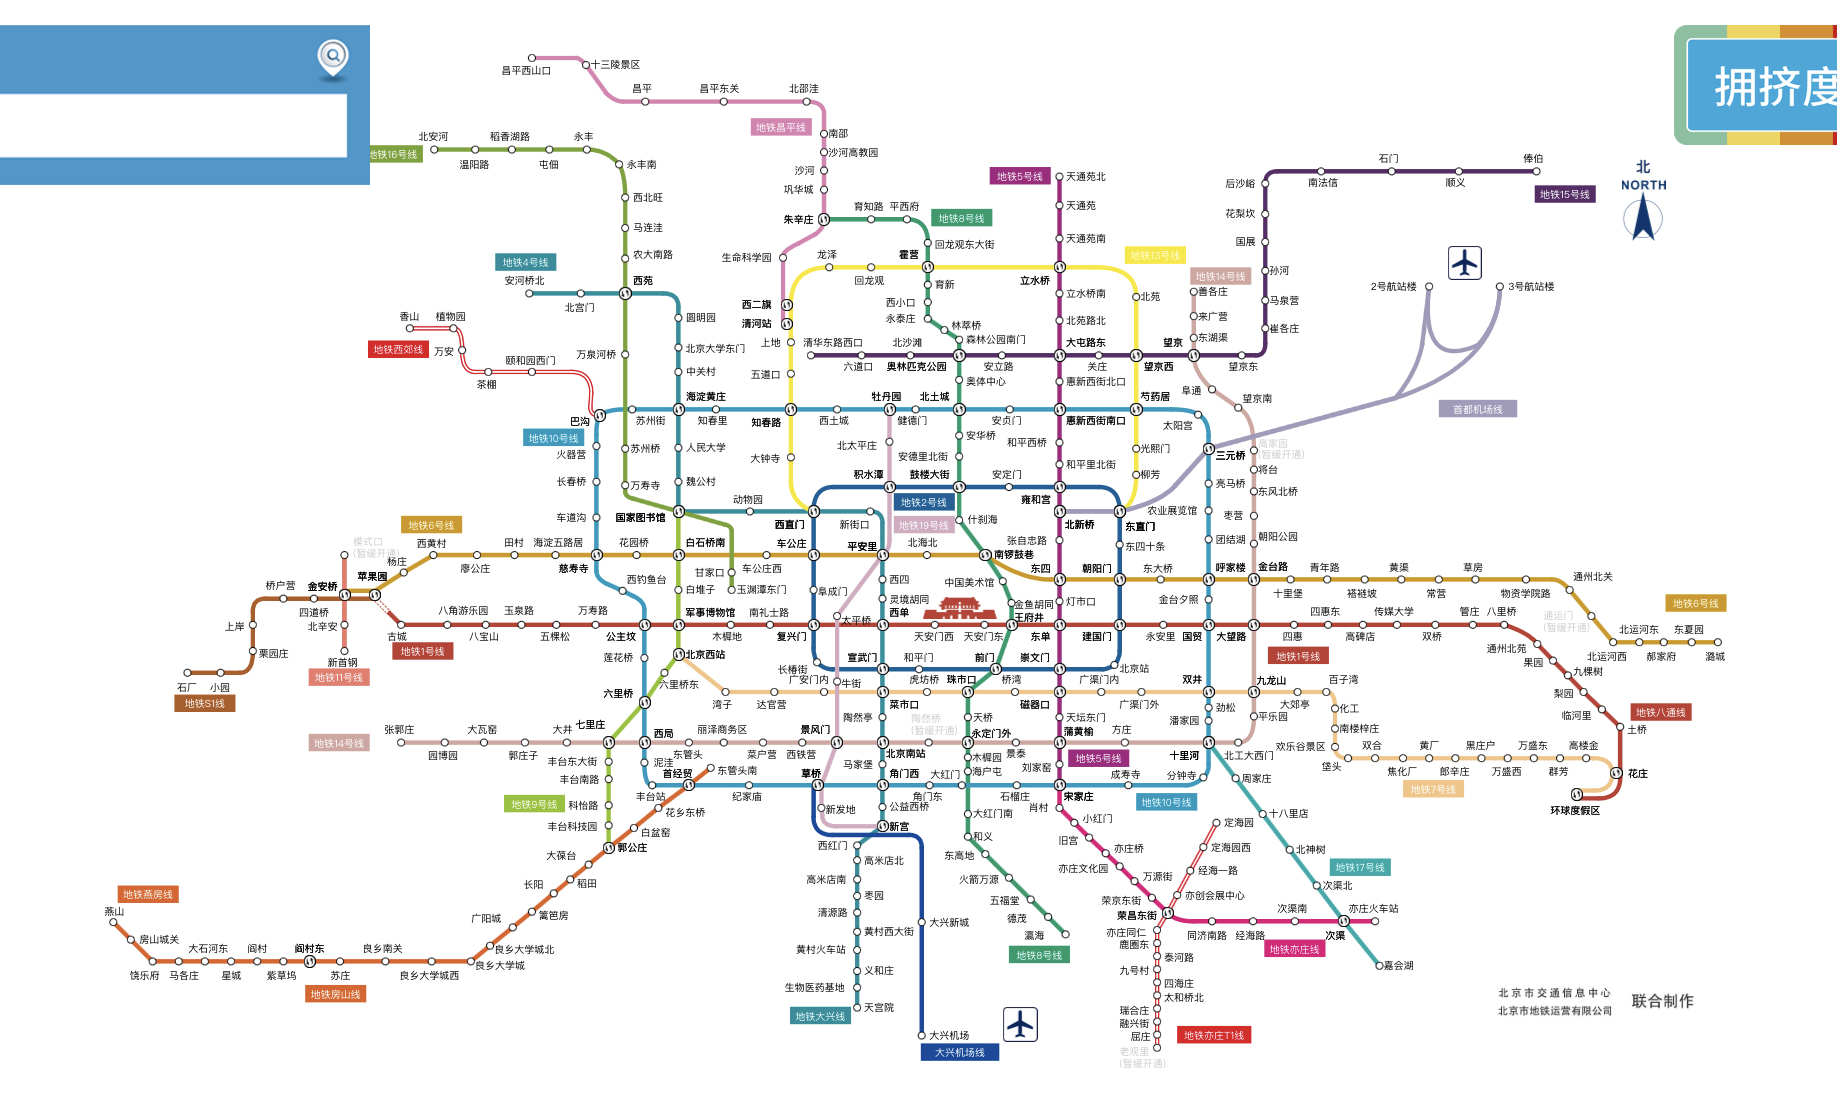
\includegraphics[width = 0.6\textwidth]{assets/bjsubway.jpeg}
    \caption{\label{fig:bjsubway.jpeg}北京地铁线路图}
\end{figure}
\subsection{地图导航}
此外,经过给定途径点的问题在生活导航中也会遇到。任两点均可不经过其他结点直达的前提过于理想化,实际上我们生活中遇到的道路规划并非如此。

如高德地图app中提供了制定包含起点、最多15个途径点、终点的路线规划功能。选择"顺路规划"则会按最短路程对途径点重新排序。

左图中1、6、7与右图中3、4、5对应。以左图标号为准,我们可以看到若需从1点直接前往7点,则必须经过6点。即这两点不可不经其他结点直达。

可惜目前这项功能还存在诸多局限性,只能对驾车进行规划、可添加的点过少。因此对于此问题,可以优化的空间还非常大,应用前景也较为广阔。
\newpage
\begin{figure}[t]
    \centering
    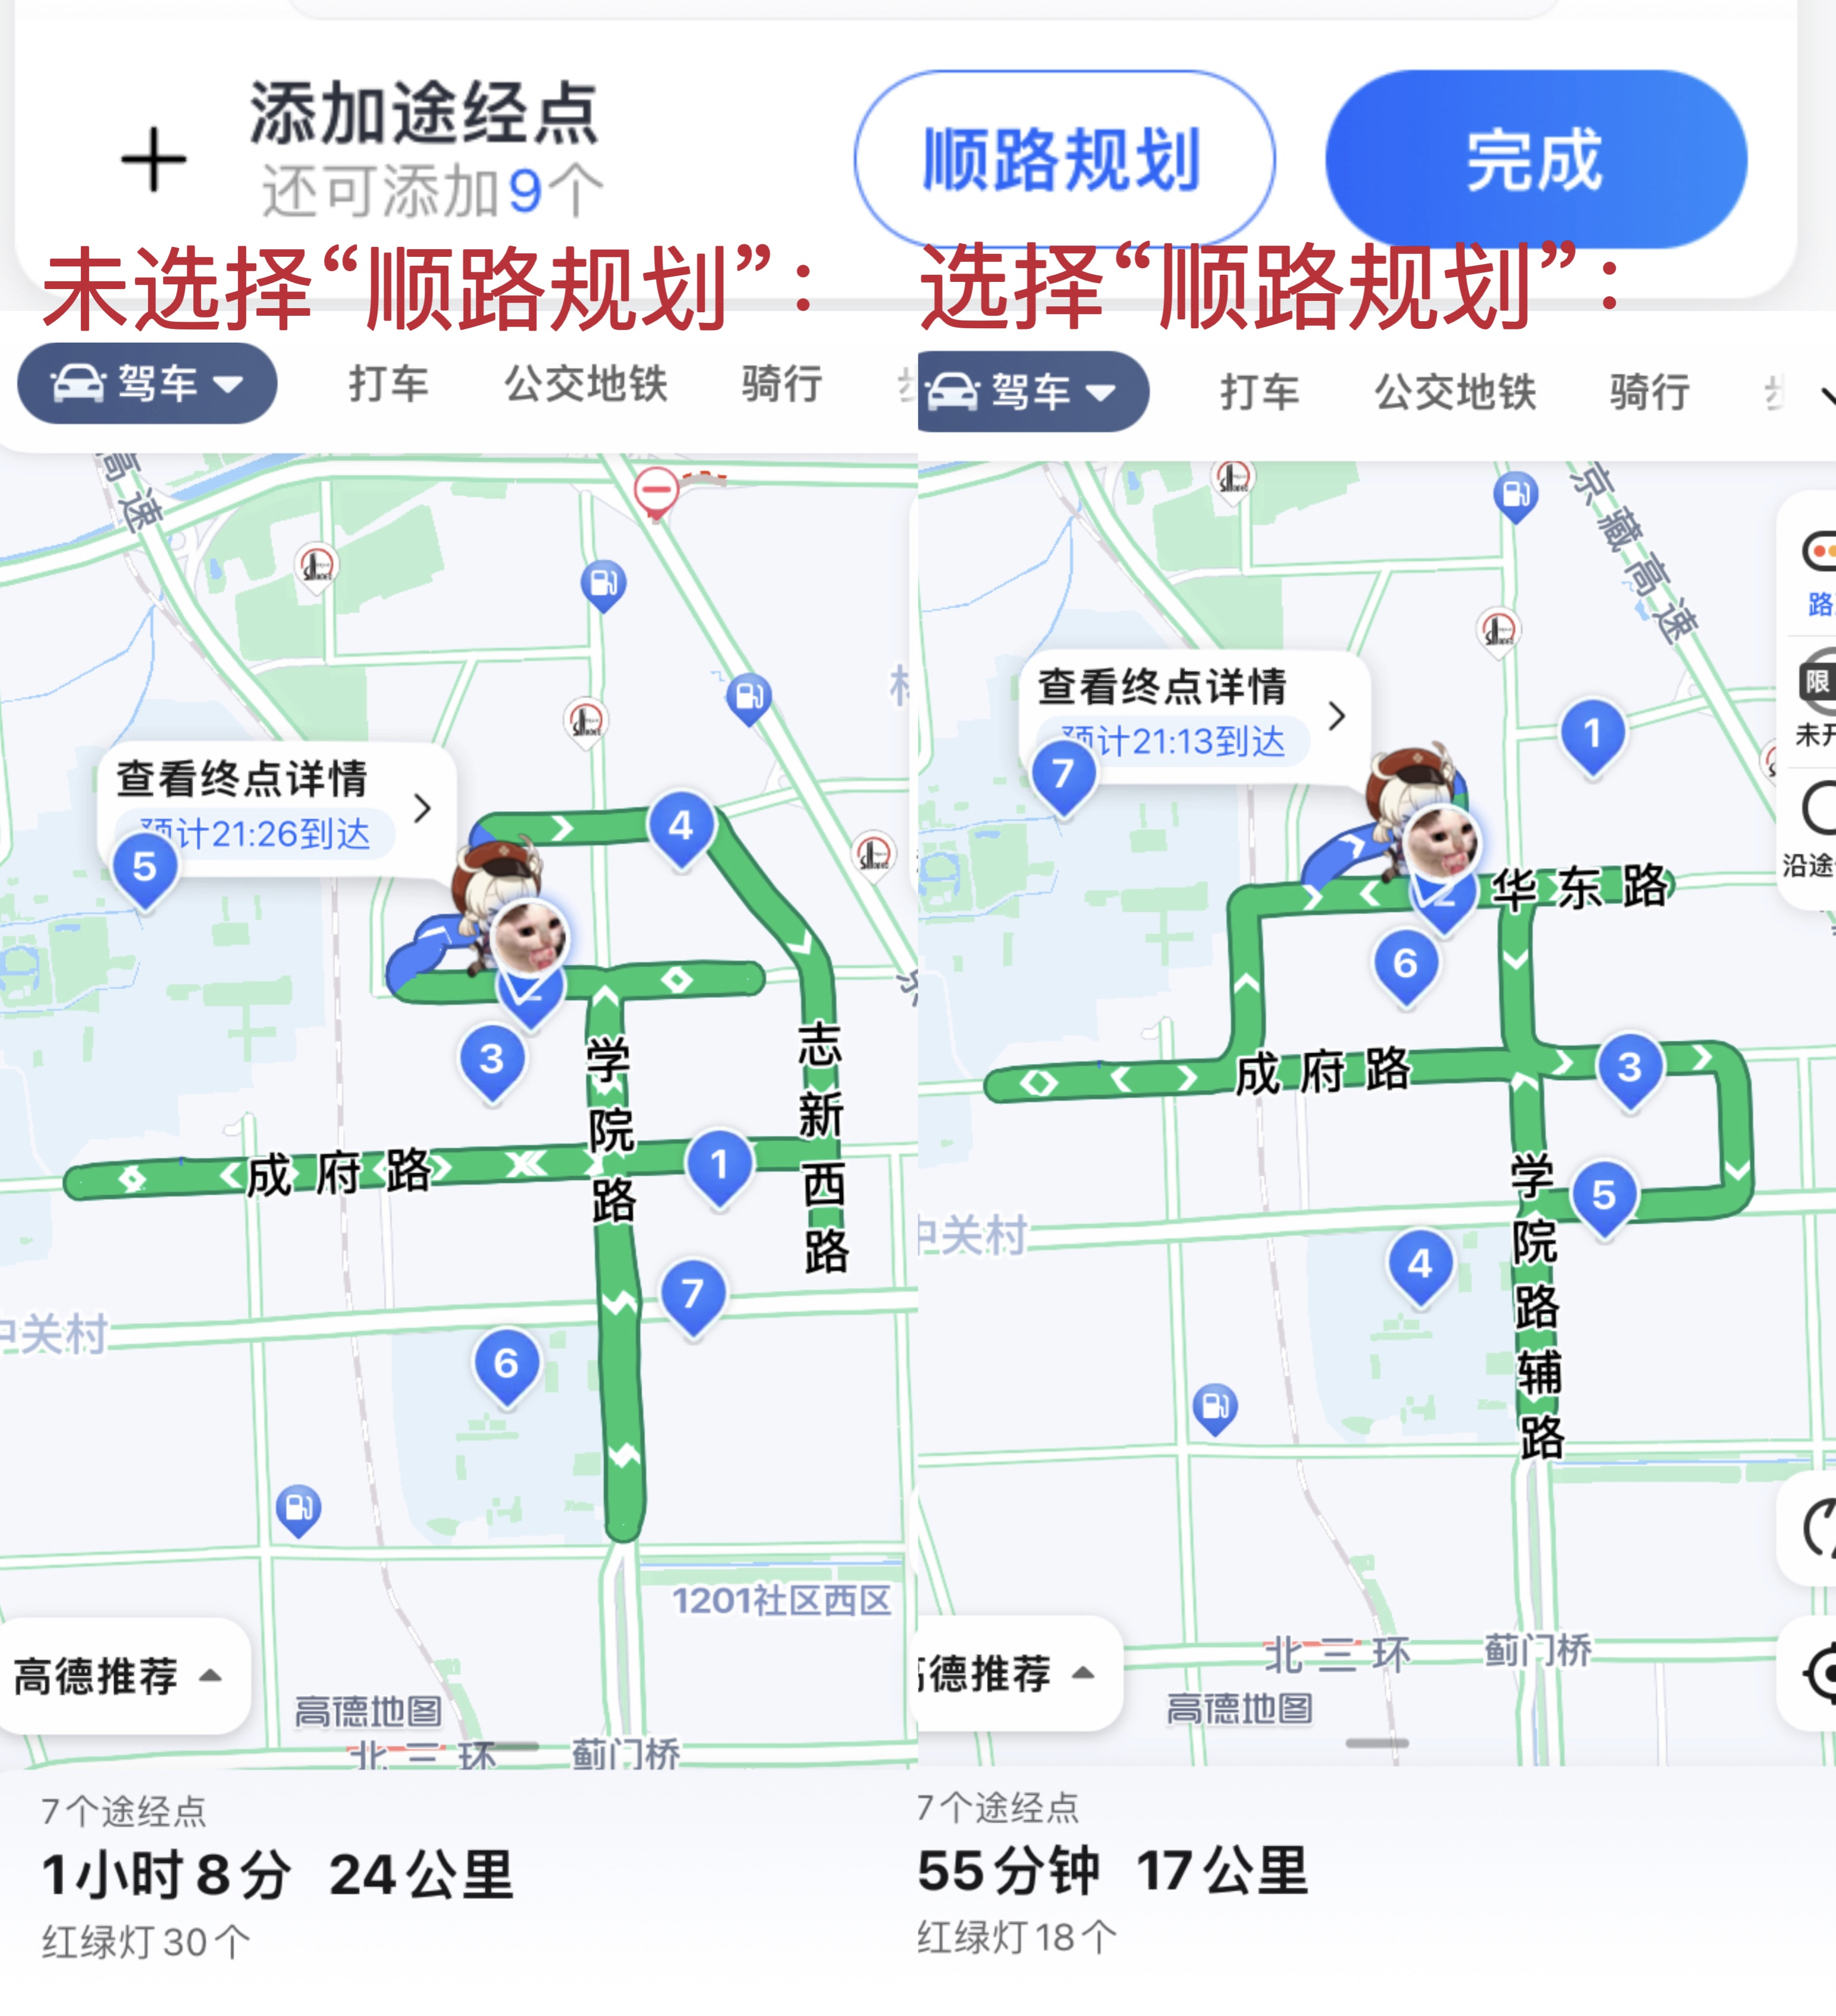
\includegraphics[width = 0.5 \textwidth]{assets/gdmap.jpeg}
    \caption{\label{fig:gdmap.jpeg}高德地图路径规划展示}
\end{figure}
~\
\newpage
\setcounter{figure}{0}

\section{模型建立与初步求解}
\subsection{问题转化}
如图2-1\footnote{绘图代码见附录1.1},定义包含权值的有向图$\mathbf{G}$,顶点集$\mathbf{V}=\{V_{1},V_{2}\cdots V_{n}\}$,必经点集$\mathbf{V'}\in\mathbf{V}$,权值集合$\mathbf{W}=\{w_{ij}\}$代表i到j点的权重。规划路线,使路线经过$\mathbf{V'}$中所有结点,并且经过的边权重和最小。

为使演示更加直观高效,示例图结点数设置较少,为11个点,后续将讨论方法的效率,以推广至多达上百、上千点的图。
\begin{figure}[htb]
    \centering
    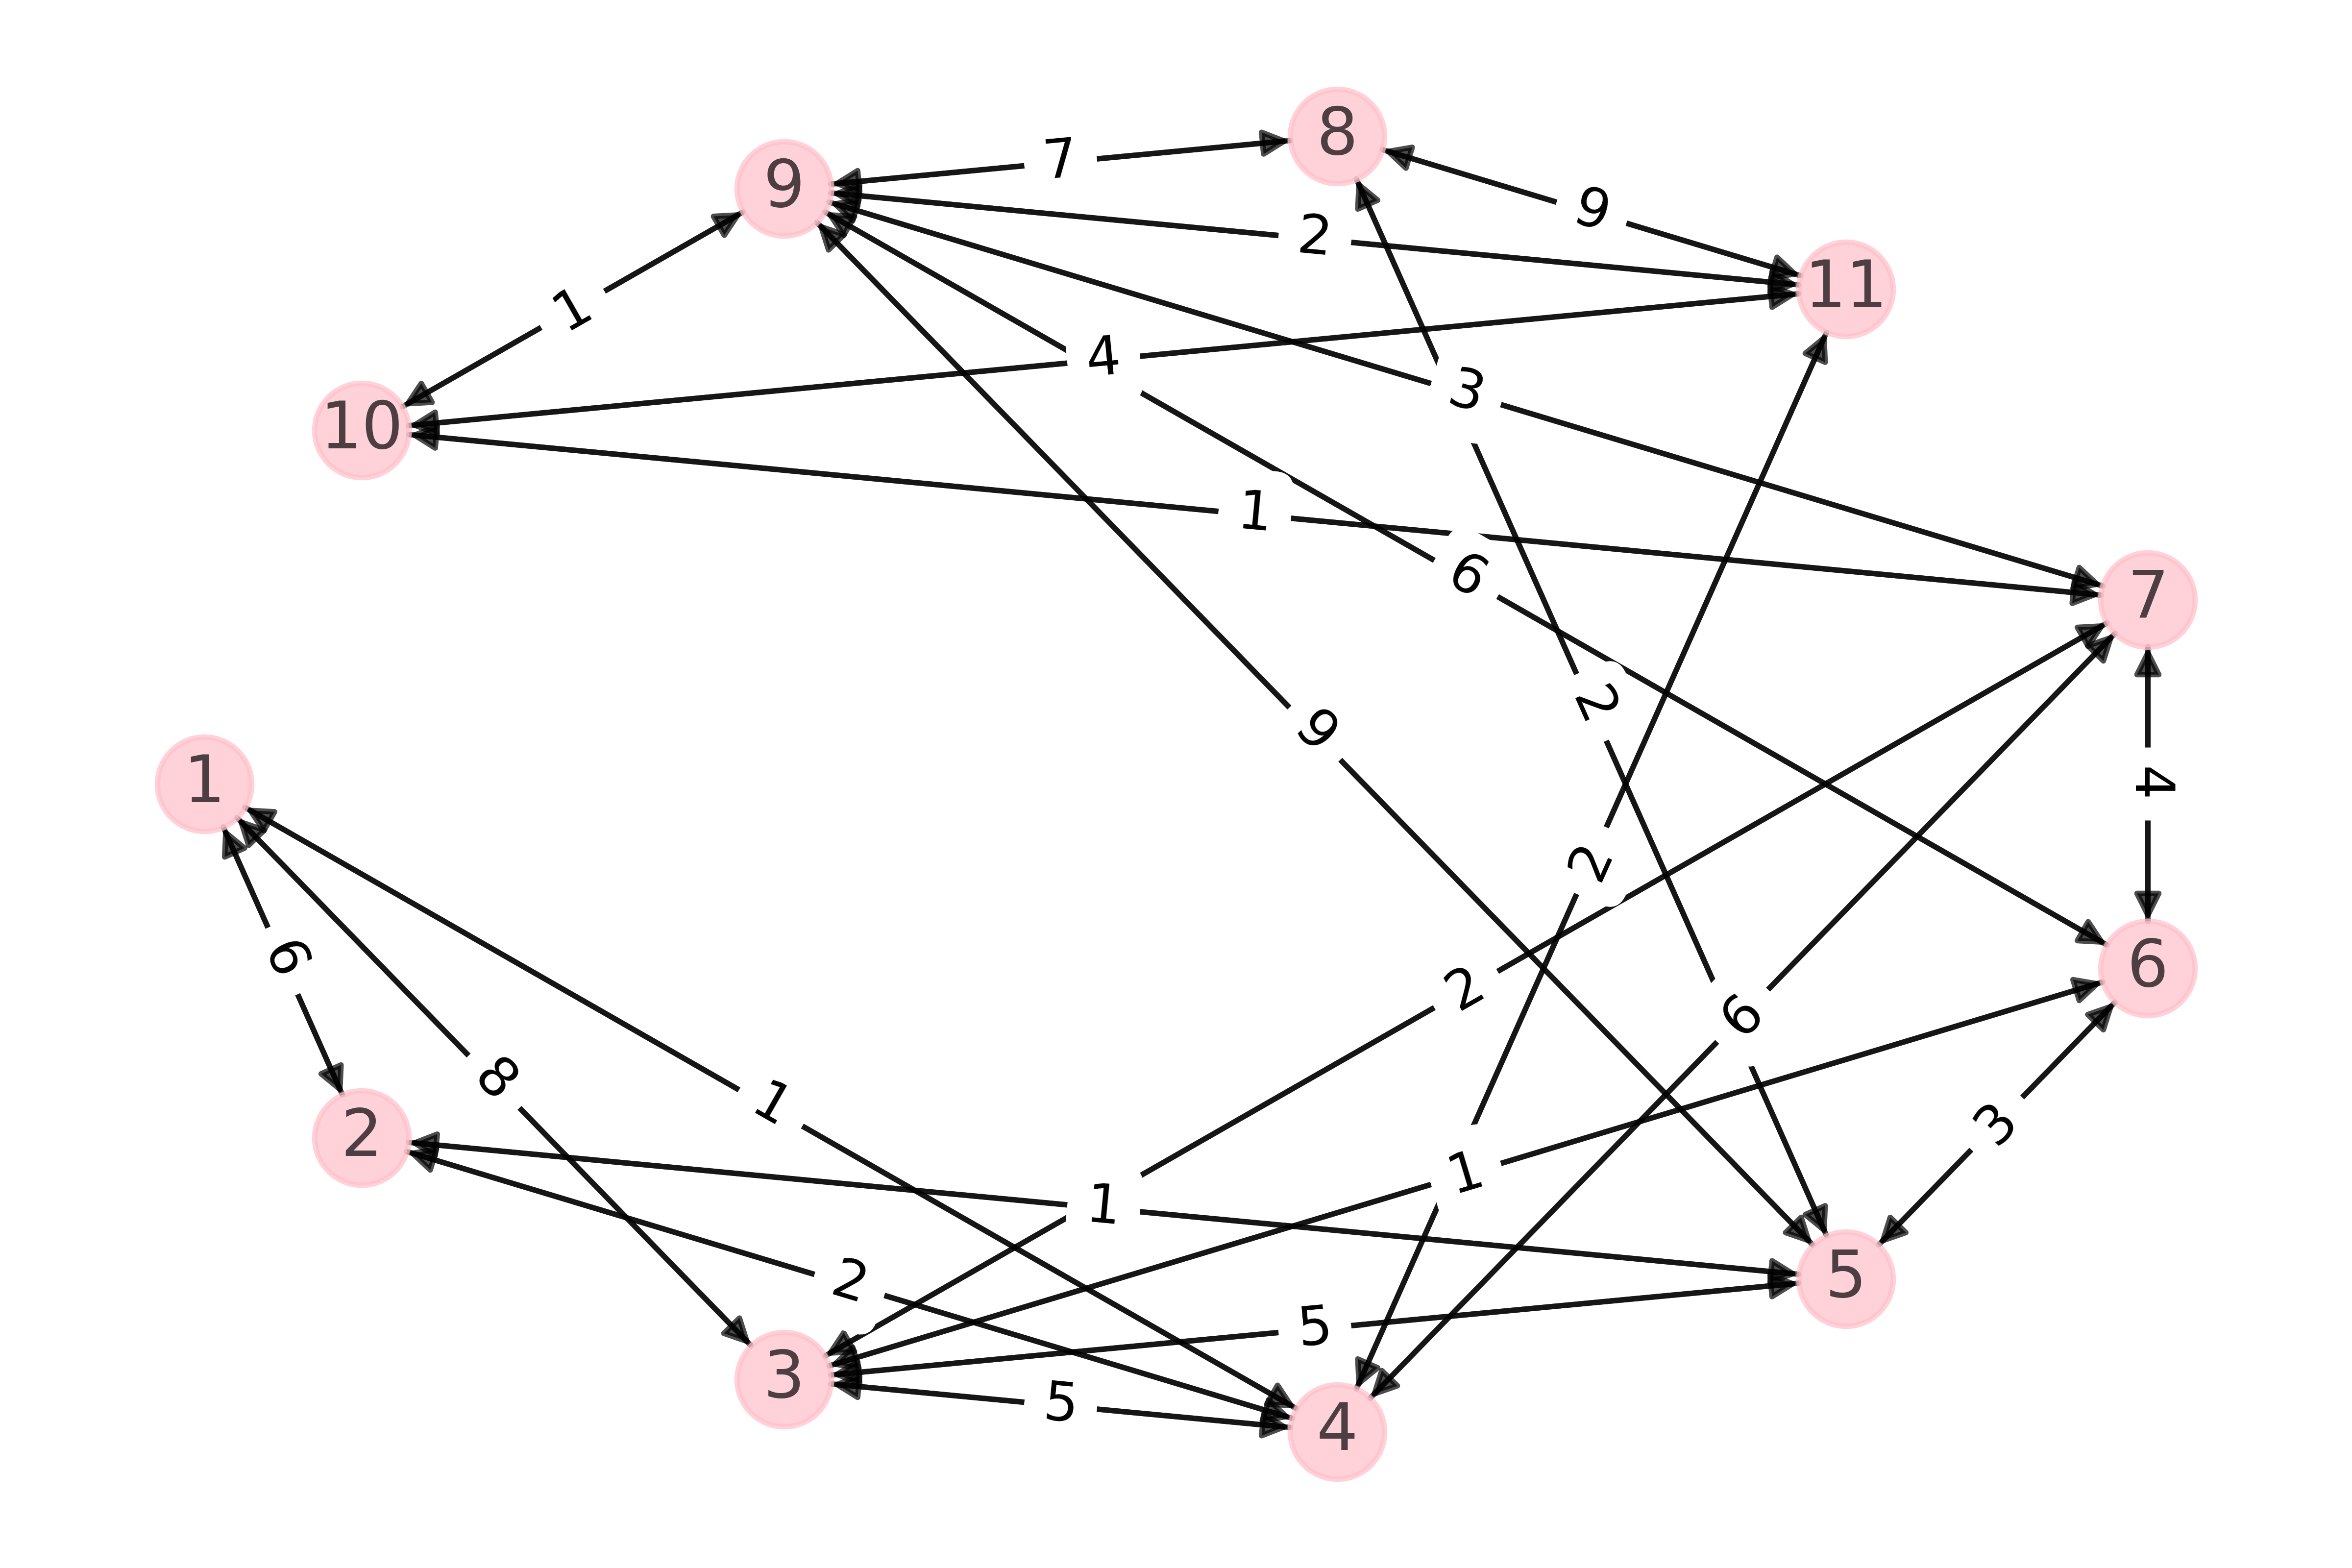
\includegraphics[width = 0.6\textwidth]{assets/graph.png}
    \caption{\label{graph.png}}
\end{figure}
\subsection{初步求解:DFS深度优先搜索}
\subsubsection{简介}
DFS(Deepth-First-Search)是计算机科学中应用非常广泛的搜索方式。其主要思想是试探及枚举来寻找最大值,从一个结点开始不断地访问其未访问的临近结点,无满足点时回溯,所有结点都访问后搜索结束。
\subsubsection{实现步骤}
图2-2示范了DFS思想的寻路步骤。蓝色表示当前所在点,紫色表示为经过点,绿色表示已经过点。

\begin{enumerate}
\renewcommand{\labelenumi}{(\theenumi)}
\item 以点1作为起始点,开始寻路。使用有序有重复的数组path记录路线,path=[1],数组visited记录已访问过的结点,visited=[1]。
\item 1的邻接点为点2,2未访问,因此访问至2,path=[1,2],visited=[1,2]。
\item2的邻接点集合为$\{3,4,5\}$,均可选择访问,此处按排列顺序进行访问至3,path=[1,2,3],visited=[1,2,3]。
\item 3的邻接点只有2,但2在visited中,因此进行回溯,直到上一个有未访问邻接点的点,即回溯至2,path=[1,2,3,2],visited=[1,2,3]。
\item 访问2的未访问邻接点4,path=[1,2,3,2,4],visited=[1,2,3,4]。
\item 4无未访问邻接点,回溯至2,path=[1,2,3,2,4,2],visited=[1,2,3,4]。
\item 访问2的未访问邻接点5,path=[1,2,3,2,4,2,5],visited=[1,2,3,4,5]。此时visited包含全部结点。此次搜索结束。
\end{enumerate}
\begin{figure}
    \centering
    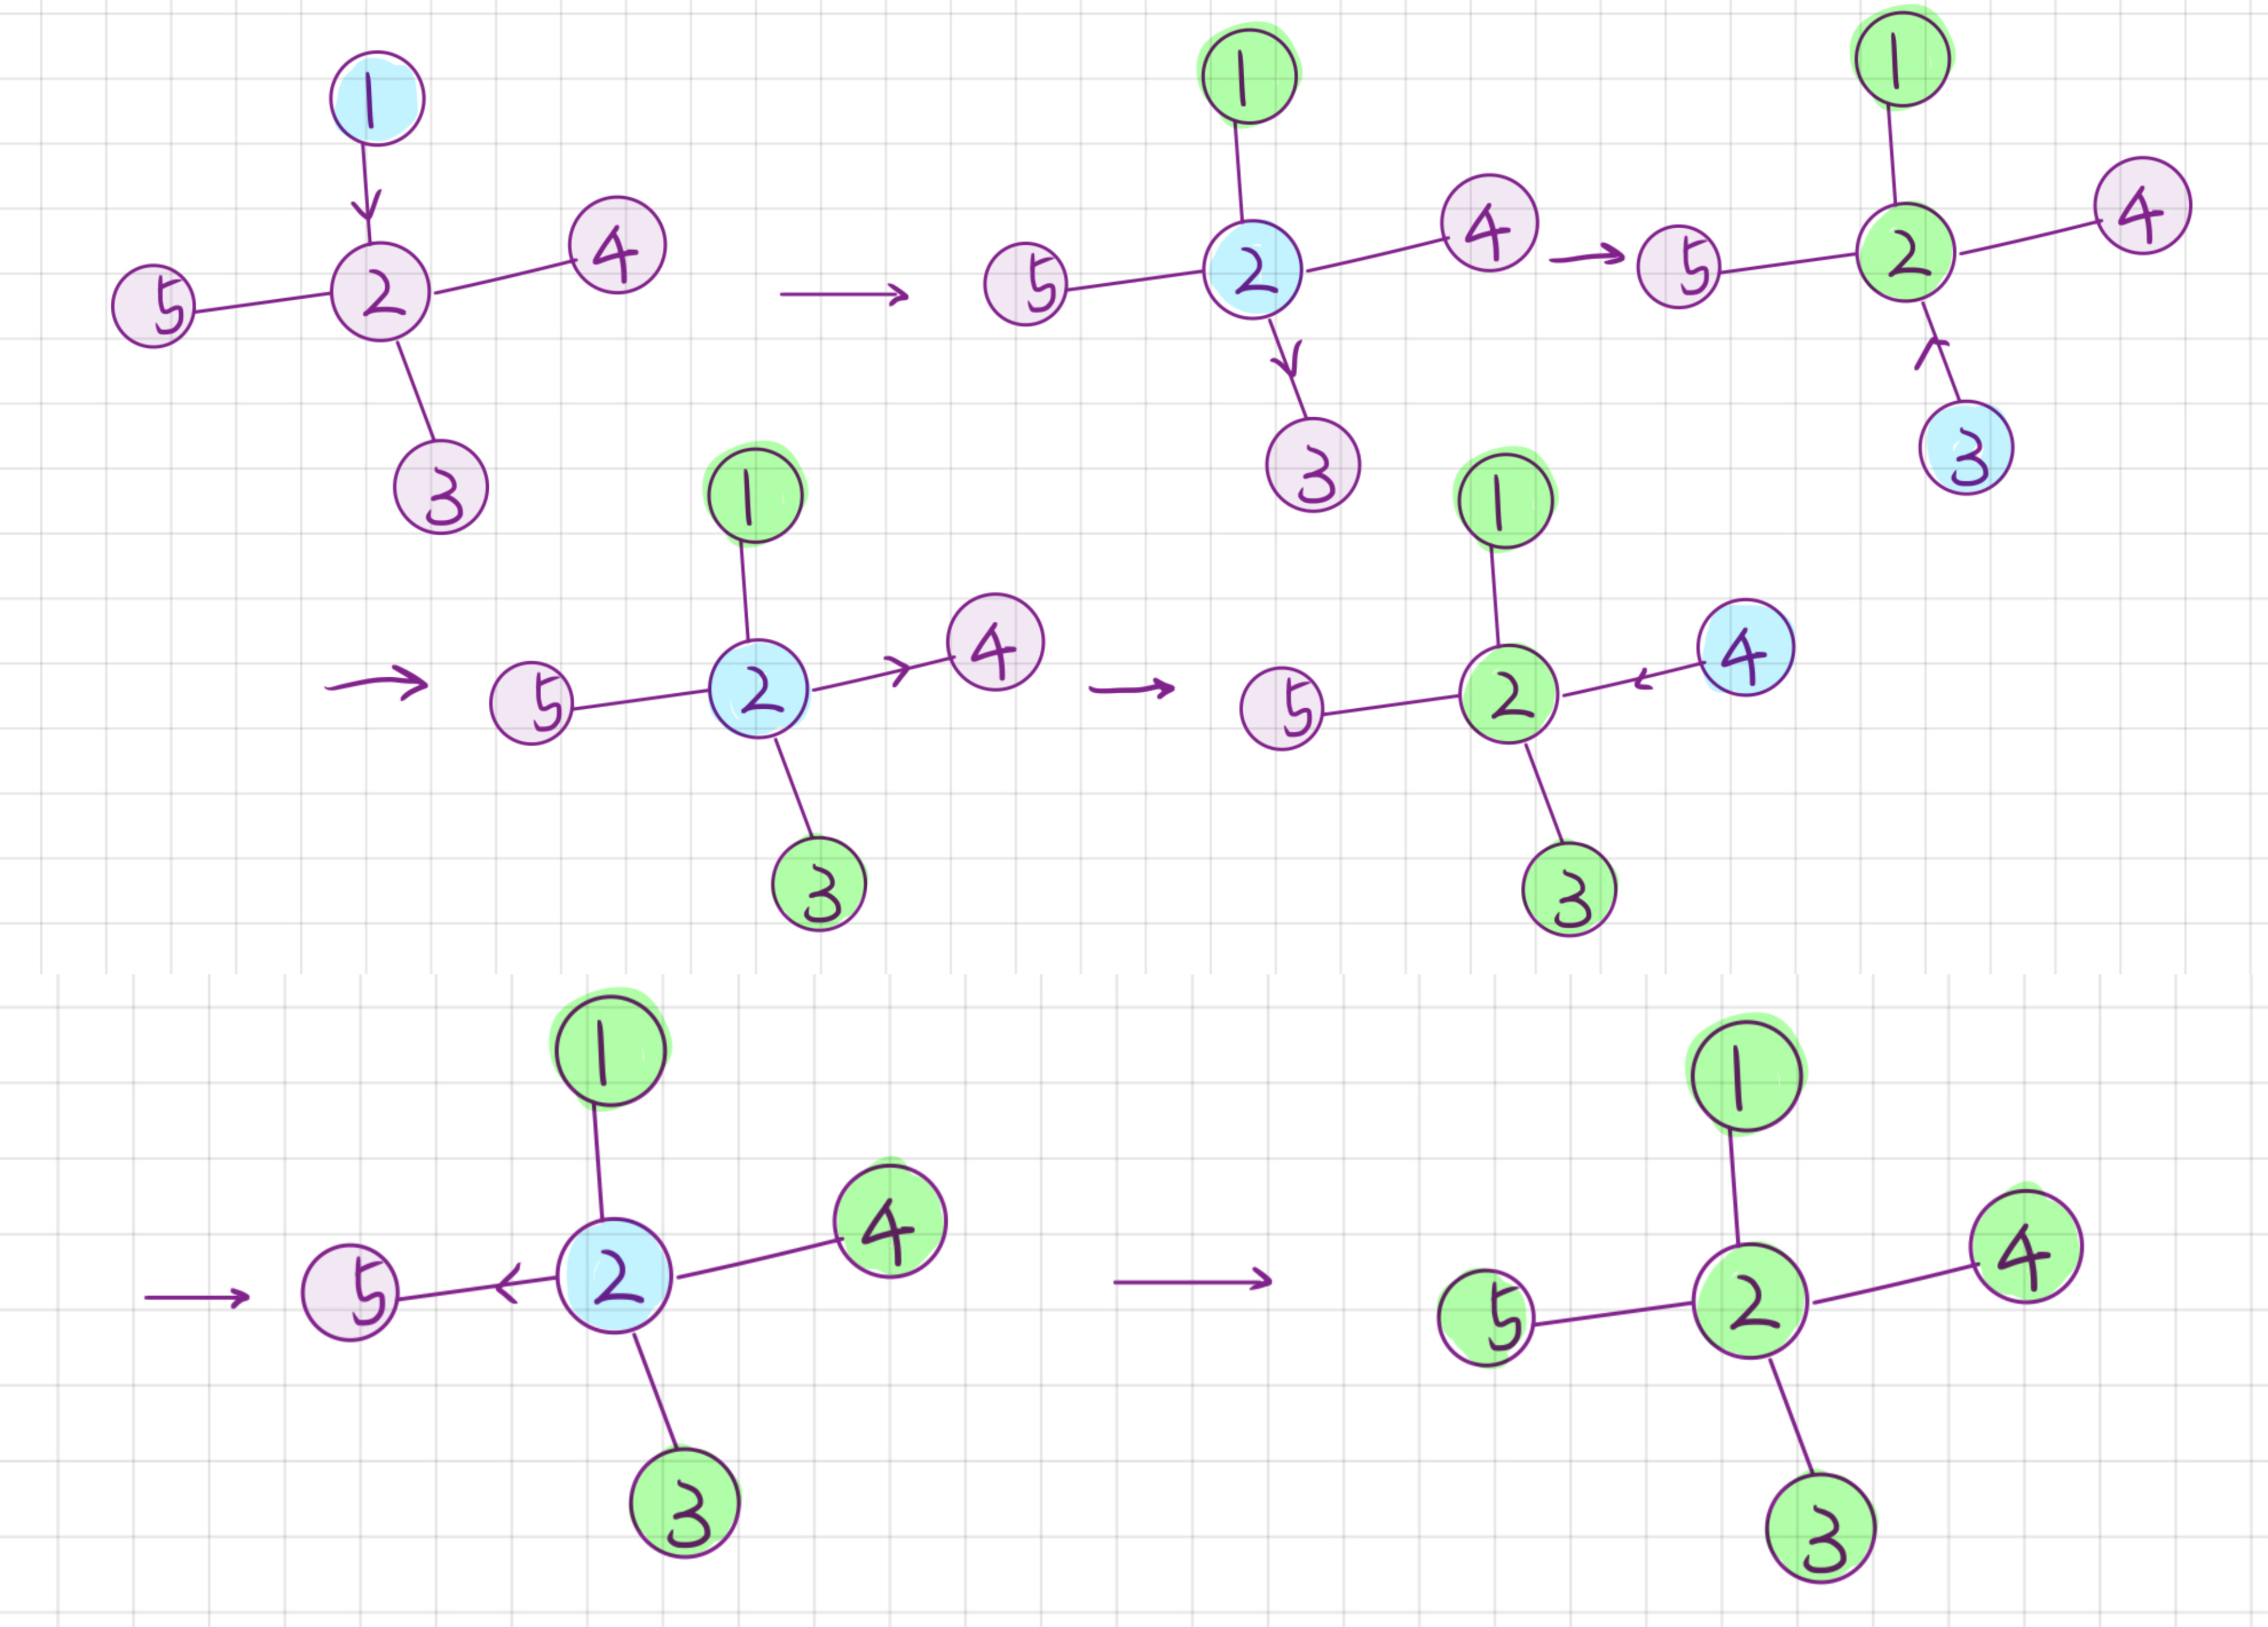
\includegraphics[width = 0.6\textwidth]{assets/dfs.JPG}
    \caption{\label{fig dfs.JPG}搜索过程图解}
\end{figure}
\subsubsection{结果}
图2-3展现了图2-1的连通情况中,必经点集合为所有点时部分可行路线。[1,0,2,4,5,6,3,
10,7,8,9]代表$2\rightarrow1\rightarrow3\rightarrow5\rightarrow6\rightarrow7\rightarrow4\rightarrow11\rightarrow8\rightarrow9\rightarrow10$。(为方便与数组编号统一减了1)
\begin{figure}[h]
    \centering
    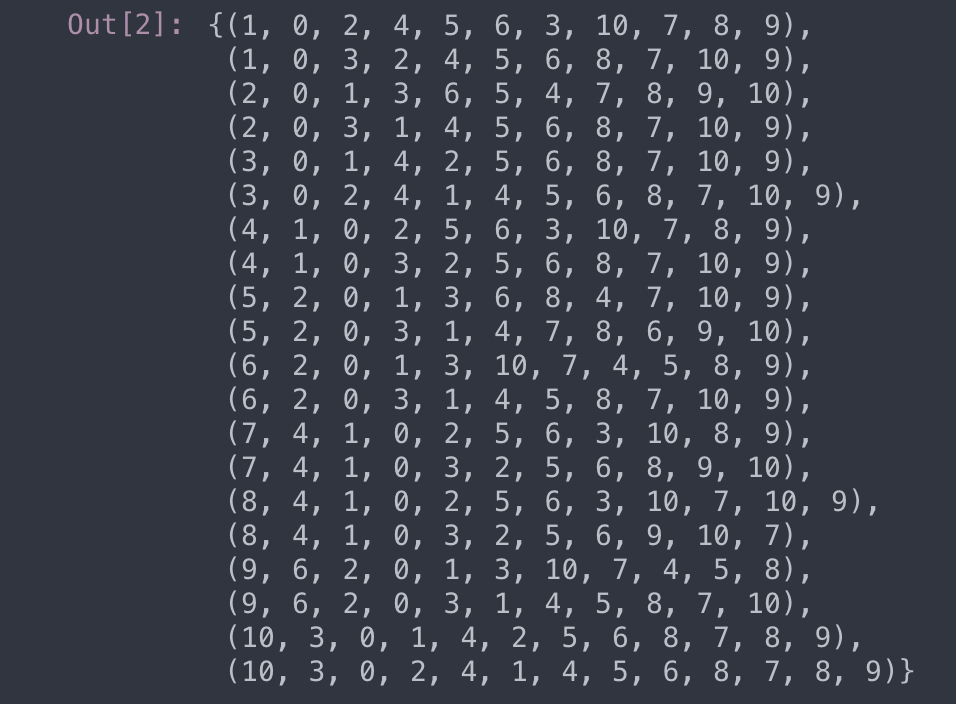
\includegraphics[width = 0.5\textwidth]{assets/possibleways.jpeg}
    \caption{\label{fig possibleways.jpeg}运行结果}
\end{figure}

若需要比较权重,使用权值集合分别加和即可。

\subsubsection{总结}
深搜方法较为暴力,但同时优点是更加精确,思路、程序简单。若在加权图中搜索最小路径,则需要将所有可能的路径距离都演算出来再进行比较,比如在一个包含n个点且每个点两两相通的图中,时间复杂度为$O(n\cdot 2^{n}) $,当点足够多时运算量非常惊人。因此需要人为进行剪枝操作来减小计算机运算量,提前剔除过长的瑕疵路线不再遍历。但这样的思路并不灵活,且仍有效率瓶颈。通常若无特定的优化,此类问题中只被用来处理30以内的点,所以不选择此方法继续深入。
\subsubsection{具体算法}
源码见附录1-2.
\begin{algorithm}[]
\caption{depth-first-search}
\LinesNumbered
\KwIn{第i次}
\KwOut{path}
def {search}(第i次)\;
    \If{path包含所有结点}{
    return path 结束搜索\;
    }
    \If{visited包含此次搜索的点所有邻接点}
        {回溯t步\;
        path.append(path[i-t])\;
        \If{visited不包含所有邻接点}
            {return {search}(第i+t次)\;
            }
        }
    \If{邻接点有不在visited中的点}
    {return {search}(i+1)\;}
\end{algorithm}
\newpage
\section{Floyd与模拟退火算法}
\subsection{思路}
本方法求解思路非常简单,对于途径点问题,可以转化为经过途径点集合$\mathbf{V'}$所有点的问题。再分别计算两点之间的最短距离,记录路径,形成最短距离矩阵,消除不连通点的影响,直接转化为传统的TSP问题,最后使用模拟退火方法进行求解。
\subsection{ 最短路径算法}
针对图中给定起点终点的最短路径,有Floyd、Dijkstra、A*、SPFA等多种方法,此处选择了Floyd继续求解,并与另一种类似算法Dijkstra进行了比较。
\setcounter{footnote}{0}
\subsubsection{Dijkstra算法}

因为课堂上学习过具体原理,本文不再深入展开,只简单介绍思想。在有向加权图G中,求点1到其他各点的最短路径方法如下:\footnote{引用自参考文献[2],见P212-214}
\begin{enumerate}
\item 定义$u_{k}$为点1到点k的最短路长度,$\mathbf{P}=\{(1,i_{1}),(i_{1},i_{2}) \dots(i_{k},j) \}$为点1到点j的有向路径,$w_{i}{j}$为点i到j的权值。
\item $u_{1}=0,u_{j}=w_{1j},(j=1,2,3\dots,n),\mathbf{P}=\{1\},\mathbf{T}=\{1,2,3\dots,n\}$
\item 指出永久编号:$\mathbf{T}$中寻找一点k,$s.t. u_{j}=min\{u_{j}\},\mathbf{P}=\mathbf{P}\cup\{k\},\mathbf{T}=\mathbf{T}-\{k\}.\mathbf{T}=\emptyset$时停止,否则转第4步。
\item 修改临时编号:$\mathbf{T}$中每一点j,$u_{j}=min\{u_{j},u_{k}+w_{kj}\}$,返回上一步。
\end{enumerate}
\subsubsection{Floyd算法}
Floyd在有向加权图G中求任两点间的最短距离矩阵方法如下:\footnote{引用自参考文献[3],见P240-241}

另权矩阵为 $\mathbf{W}=\left(d_{i j}\right)_{n \times n}, w_{i j}$ 为 $v_i$ 到 $v_j$ 的距离。
其中
$$
d_{i j}= \begin{cases}w_{i j} & \text { 当 }\left(v_i, v_j\right) \in E \\ \infty & \text { 其他 }\end{cases}
$$
\begin{enumerate}
\item 输人权矩阵 $\mathbf{W}^{(0)}=\mathbf{W}$ 。
\item 计算 $\mathbf{W}^{(k)}=\left(d_{i j}^{(k)}\right)_{n \times n} \quad(k=1,2,3, \cdots, n)$
其中 $\quad d_{i j}^{(k)}=\min \left[d_{i j}^{(k-1)}, d_{i k}^{(k-1)}+d_{k j}^{(k-1)}\right]$
\item 迭代n次后,$\mathbf{W}^{(n)}=\left(d_{i j}^{(n)}\right)_{n \times n}$ 中元素 $d_{i j}^{(n)}$ 就是 $v_i$ 到 $v_j$ 的最短路长。
\end{enumerate}
\subsubsection{效率比较}
另外几种最短路径方法本文没有深入研究,仅供比较了解:
\begin{table}\centering

\begin{tabular}{ccccc}
  \toprule
\cmidrule{1-4}
& Dijkstra & Floyd & A* & SPFA(Bellman-Ford)\\
  \midrule
& 单源最短路径 & 任两点最短路径矩阵 & 大规模问题 & 含负权边问题\\
 & \makecell[c]{$O(n^{2})$\\ 堆优化$O(nlog_{2}n)$}  & $O(n^{3})$ & $O(n^{2}log_{2}n)$ &  \makecell[c]{最坏时$O(VE)$ \\V、E 为顶点和边的数量} \\
&\makecell[c]{不能处理负权 \\ 适合稀疏图} & \makecell[c]{可处理负权\\ 适合稠密图} & \makecell[c]{启发式算法\\可能只找到局部最优} &\makecell[c]{效率不稳定\\可能很低} \\
  \bottomrule
\end{tabular}
\end{table}

由于floyd方法编写简单,也更适合本题需要的最短距离矩阵,选用floyd进行研究。以下是随机生成点的运行效率测试:\footnote{源码见附录1-4.}

\begin{tabular}{ccccc}
 \toprule
\cmidrule{1-4}
& node & 50个点 & 300个点 & 500个点\\
  \midrule
& time(s) & 0.0136 & 2.3062 & 11.1489\\
    \bottomrule
\end{tabular}

在已知图G的连通情况和权值时,我们可以生成其最短路径矩阵D。对图2-1展示的图,最短路径矩阵为\footnote{篇幅有限,详见附录}
\[ \mathbf{D} = \left( \begin{array}{ccccc}
0 & 3 & 6 &\ldots & 3\\ 3 & 0 & 5 &\ldots &4\\ 
\vdots & \vdots & \vdots  & \ddots  & \vdots
\\3 & 4 & 6 & \ldots & 0\\ \end{array} \right) \]。
\subsection{模拟退火原理}
\subsubsection{简介}
模拟退火(Simulate Anneal,SA)是一种基于概率的随机优化算法,也就是说当问题规模足够大时,如果迭代次数不够多,能否生成最终的精确结果需要看运气,可能只能在最优解附近徘徊。模拟退火的思想来自于模拟固体加热到一定温度后降温的过程。

许多教程把这些优化算法都说得比较晦涩难懂,一上来就引入很多代词,使读者\footnote{特指脑子反应比较慢的我}抓不到重点,看了很多次才看懂,所以我尝试以比较通俗的方式自己来解释一下模拟退火方法。

模拟退火是怎么与优化联系起来的呢?我们可以想象一下物理学中高温物体其粒子是无序的、不稳定的,而当其降温至常温时,其粒子排序趋于稳定态。这个类比的重点就是把高温物体的粒子排序看作是待优化的初始解,而稳定态下的常温模型就是经过一定优化过程后的最优解,我们将其推广到我们面临的待优化问题上,这个优化过程便是模仿粒子运动来实现的。

优化过程可以看作是不断地寻找降温、即向着更优的方法,不断生成新解,依靠一定的准则来选择此解是否更优进行迭代,也就是降温。接下来将结合TSP问题讲述模拟退火是怎么实现找到最优解的。
\subsubsection{评价函数}
顾名思义,评价函数就是对当前解进行评价,在退火过程中,内能高的结果是较差的,内能低的是我们想要的较好的,这个内能高低就是评价准则。在寻找最优路径的过程中,评价函数就是计算路径的总长度的函数,以此来给出优劣判断,路径长的结果是较差的,能量高;路径短的结果是较好的,能量低。我们使用$E_{k}$来表示k状态的能量,也就是k状态收到的量化评价。
\subsubsection{生成新解}
模拟退火法的基本思想和蒙特卡罗随机概率法类似,在不强调效率优化的情况下,对新解的迭代只要使用任意随机算法即可。在寻路问题中我采用的方法是:随机选取路径中任意两点进行交换。
\subsubsection{Metropolis接受准则}
Metropolis接受准则的核心思想就是以一定概率接受比当前解较差的解,更新当前解。模拟退火使用了这样的方法来跳脱出局部最优,避免无法随机到全局最优的点。

\setcounter{figure}{0}
比如在3-1图中需求函数的最小值,不采用一切较差点的结果是,可能在b点处就结束了搜索,认为得到了最优解。而接受较差点使程序可以继续往d点移动,直到达到全局最优。
\begin{figure}[h]
    \centering
    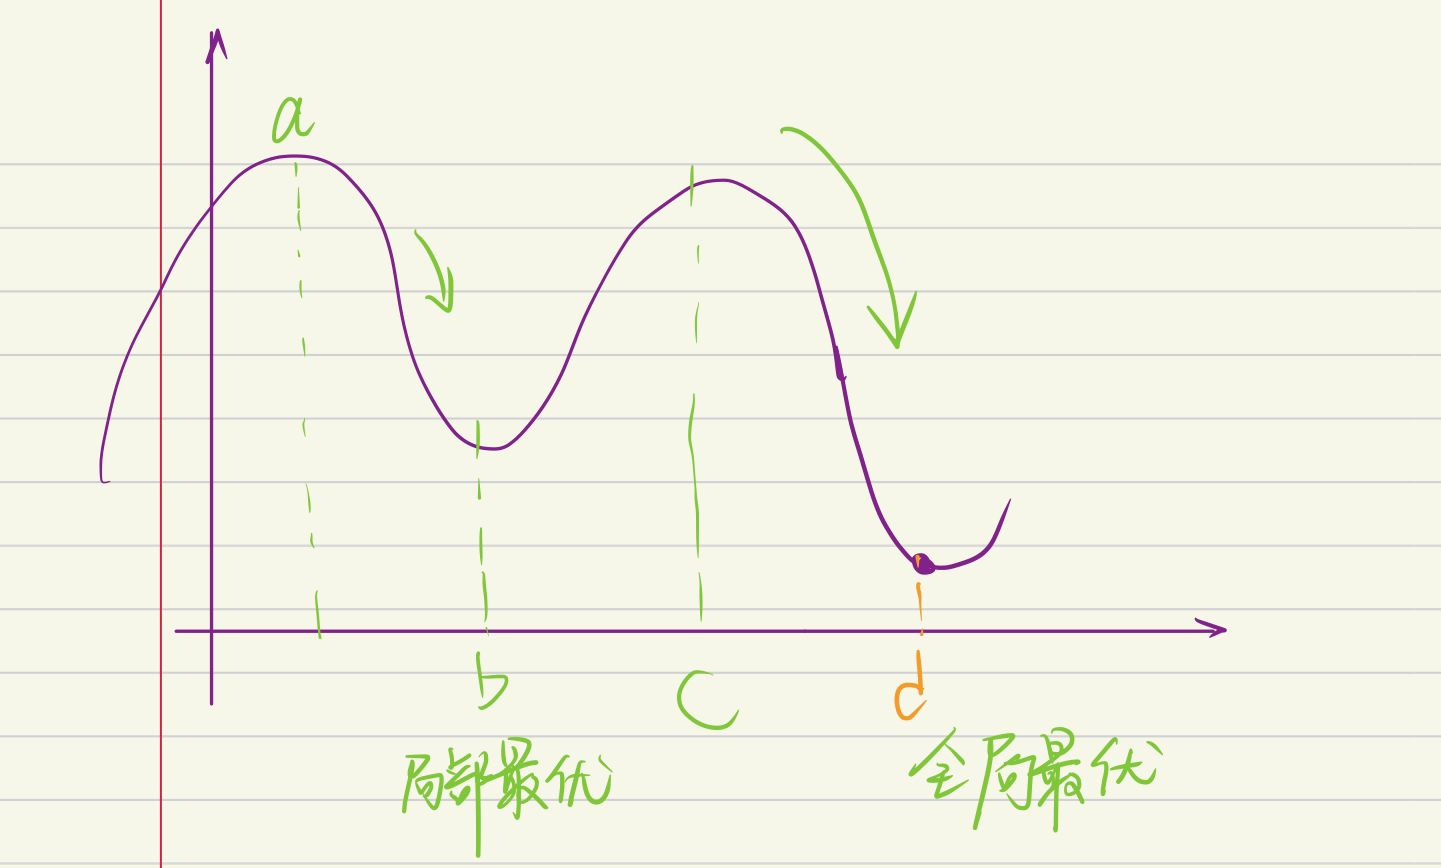
\includegraphics[width = 0.5\textwidth]{assets/Metropolis-examp.jpg}
    \caption{\label{fig Metropolis-examp.jpg}接受准则示例}
\end{figure}

从状态k转移到状态j时,这个概率可以写为:
\[ P=
\begin{cases}
e^{-\frac{\varDelta E}{T}} & \text{if } E_{j}\ge E_{k},\\ 
1 & \text{if } E_{j}<E_{k}.
\end{cases} \]
其中$\varDelta E=E_{j}-E_{k},$T代表当前温度。这个函数的规律表示温度较高,即迭代刚开始时,接受较差解的概率越高;温度越低,即迭代快结束时,接受较差解的概率越低。
\subsubsection{初始化}
模拟退火方法需要多个变量参与运算。代表降温过程的变量:初始温度$T_{0}$,终止温度$T\prime$,每个温度的迭代次数(也被称为马科尔夫链长)L,降温速率v,当前温度t。

其次需要定义一个初始解,越接近最优解,得到精确结果的可能性就越大。在不要求特别精确的情况下,我们可以直接随机生成,比如初始路线就设为[1,2,$\cdots$n].但需要注意,初始解必须是可行解。

评价函数在最优路径问题中就是计算当前路径的距离。在上述D矩阵中,$\sum_{i=1}^n d_{i,i+1}$代表了当前路径的距离.
\subsubsection{温度状态}
接下来介绍代表当前状态的温度,温度的计算方法为,从初始温度开始,在温度t时迭代L次降温至t·v,直到t$\le T\prime$停止。因此总共的迭代次数为$log_{v}\frac{T\prime}{T_{0}}$. 

比如当设计$T_{0}=1000$,$T\prime=10^{-3}$,链长250时,总共的迭代次数约为30000次,对于多达几百点的问题已经可以得到较为精确的解,相比于动态规划、DFS的复杂度$O(n\cdot 2^{n})$,已经大大优化了运行难度。理论上来说,v越接近1,链长越长,搜索会越充分,但效率更低。
\subsection{实现流程}
$input$:邻接矩阵G;$output$:最短路径path
\begin{enumerate}
	\item 使用floyd算法得到最短距离矩阵D,最短距离路线矩阵$D_{p}$存储每条最短距离路线。
	\item 开始进行模拟退火,生成初始解p,计算初始距离。
	\item 产生新解并计算距离,评价优劣。若新解更短则更新状态,更长则按Metropolis接受准则选择更新状态。
	\item 第三步迭代L次后降温,令新t=t·v。
	\item 重复迭代降温,直到温度达到最低温后停止。输出此时的状态最短路径path。
\end{enumerate}
\subsection{结果与改进}
\begin{figure}[h]
    \centering
    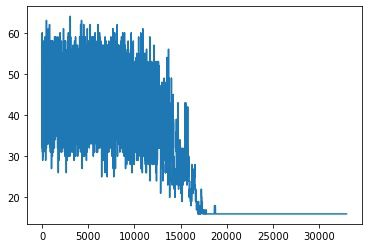
\includegraphics[width = 0.5\textwidth]{assets/evolution.jpg}
    \caption{\label{fig evolution.jpg}进化过程}
\end{figure}
\subsubsection{结果}
对示例图2-1,按照上节温度状态的示例方法定义迭代次数,所得经过所有点且路程最短的路径为: [8, 5, 2, 4, 1, 4, 11, 9, 10, 7, 3, 6],[6, 3, 7, 10, 9, 11, 4, 1, 4, 2, 5, 8],长度为16.图3-2展示了迭代的过程。

\subsubsection{改进}
(这里并没有优化算法的效率,只是扩展了算法的应用进行了一些小改动。)
\begin{enumerate}
\item 记录满足条件的路径

例:在示例图2-1中保存过所有点且满足权值和小于等于20的路径

声明set以防止路线重复,判断条件加入set中,写在SA函数的定义里。
\begin{lstlisting}
	res = set() #存储路径
	if total_distance <= 20:
           res.add(tuple(path))
\end{lstlisting}
\item 扩展路径表达

直接套用tsp解法的SA算法不能生成完整的路径,需要借用先前存储的$D_{p}$矩阵将路线展开。
\begin{lstlisting}
	pp = []
    for i in range(len(path)-1):
          tempp=shortp[path[i]-1][path[i+1]-1]
           for n in range(0,len(tempp)-1):
               pp.append(tempp[n])
    pp.append(path[len(path)-1])
\end{lstlisting}
\item 指定起点终点

例:起点为2,终点为3.在选定初始解时定好起点终点,并且生成新解时固定两点。
\begin{lstlisting}
#初始化处增加语句
lst_s = [2,3]
lst_t = [i for i in range(1,len(distance)+1)]
lst_t.remove(len(distance))
lst_t.remove(1)
#生成初始解处修改为任意满足条件可行解,如
path=[2,1,4,5,6,7,8,9,10,11,3]
#生成新解处修改
idx1 = random.sample(lst_t,1)[0] -1
idx2 = random.sample(lst_t,1)[0] -1
\end{lstlisting}
结果:最优路径 [2, 8, 5, 4, 1, 11, 9, 10, 7, 6, 3],距离20.
\item 修改途径点

直接改初始解即可,使初始解包含且仅包含所有途径点。
\end{enumerate}
\subsection{效率与总结}
关于模拟退火的运行效率仅和迭代次数、距离计算有关,比如3万次的迭代、11点的加和比较约为30万次的计算量,300点的加和大概就是900万次,总体消耗时间很少。
使用random函数随机生成距离矩阵进行了简单的效率测试(不计算生成距离矩阵的时间,仅计算退火时间):


\begin{enumerate}
	\item 依据3.3.6示例的温度参数,400点运行时间为5.296s,初始距离由2309优化至667.由进化图可见迭代次数较少,最后结果并未趋于稳定,只是靠近最优解。
	
	在b图中,我尝试了改变初始解来优化收敛时间,但退火生成新解是完全随机的,与初始解的好坏与否无关,所以结果并未优化。
\begin{figure}[htbp]
\centering
\subfloat[]{
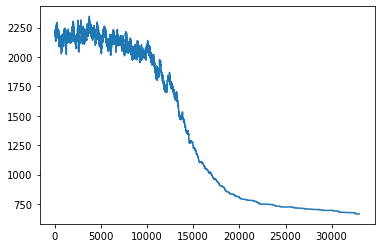
\includegraphics[width=5.5cm]{assets/400-1-evolution.PNG}

}
\quad
\subfloat[]{
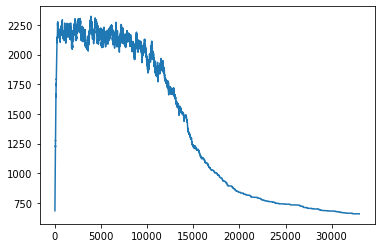
\includegraphics[width=5.5cm]{assets/400-2-evolu.PNG}
}
\quad
\subfloat[]{
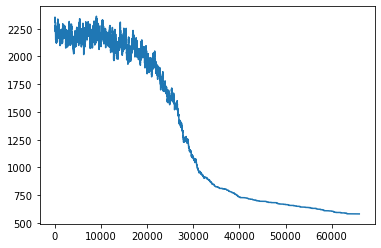
\includegraphics[width=5.5cm]{assets/400-3-evolu.PNG}
}
\quad
\subfloat[]{
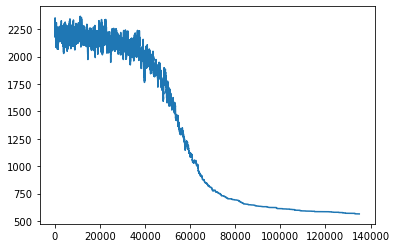
\includegraphics[width=5.5cm]{assets/400-4-evolu.PNG}
}
\caption{400点进化过程}
\end{figure}
\item 其他数值不变,仅改变链长为500,使迭代次数翻倍。运行时间为10.22s,最佳距离582,如图c。
\item 再上一条的基础上将降温速率变为0.95,运行时间20.402s,最佳距离564,如图d。
\end{enumerate}

由上述简单的实验过程可见,仅通过改变温度计算方法等手段增加迭代次数,确实可以达到想要的更精确的解,但迭代的过程,也就是进化图的形状在同比例下是类似的(为了使结果更加直观,图片大小相同,因此坐标系的尺度是不一样的)。可见这样并没有对算法进行实际上的优化,只是单纯地增加了运算次数。

其实对于这个方法已经基本可以解得我想要的结果了,对几百点这种规模较大的,只需得到大致的解的话运行效率在15秒左右,可以接受。可惜的是模拟退火还是受限于随机性,上面举的11点例子都会出现没有得到最优解的情况,需要多次重复运行或者增加迭代数,降低效率,但仍不能完全保证解的正确性,对于怎么生成新解等等都有很大的优化空间。

个人认为这个方法还不是特别灵活,我也尝试过不用求出最短路矩阵直接使用优化算法寻路,但由于每次走过的点步数、次数都不能保证,苦恼于不能生成新的可行解,遂放弃。因此我找到了蚁群算法,旨在直接进行寻路,希望能对其效率和灵活性进行优化。
\newpage
\section{蚁群算法}
针对一般的蚁群算法,为使其可以经过所有途径点,我的思路是加以终止条件约束,当所有必经点被经过时停止,并且对蚂蚁选择路径的过程进行修改。蚂蚁可以重复访问一个点,但不能重复经过两点间连通的一条有方向的路。由于时间有限,此方法暂时没有落地实现,只是提供了思路方向和可行性分析。
\subsection{简介}
\setcounter{figure}{0}
\begin{figure}[h]
    \centering
    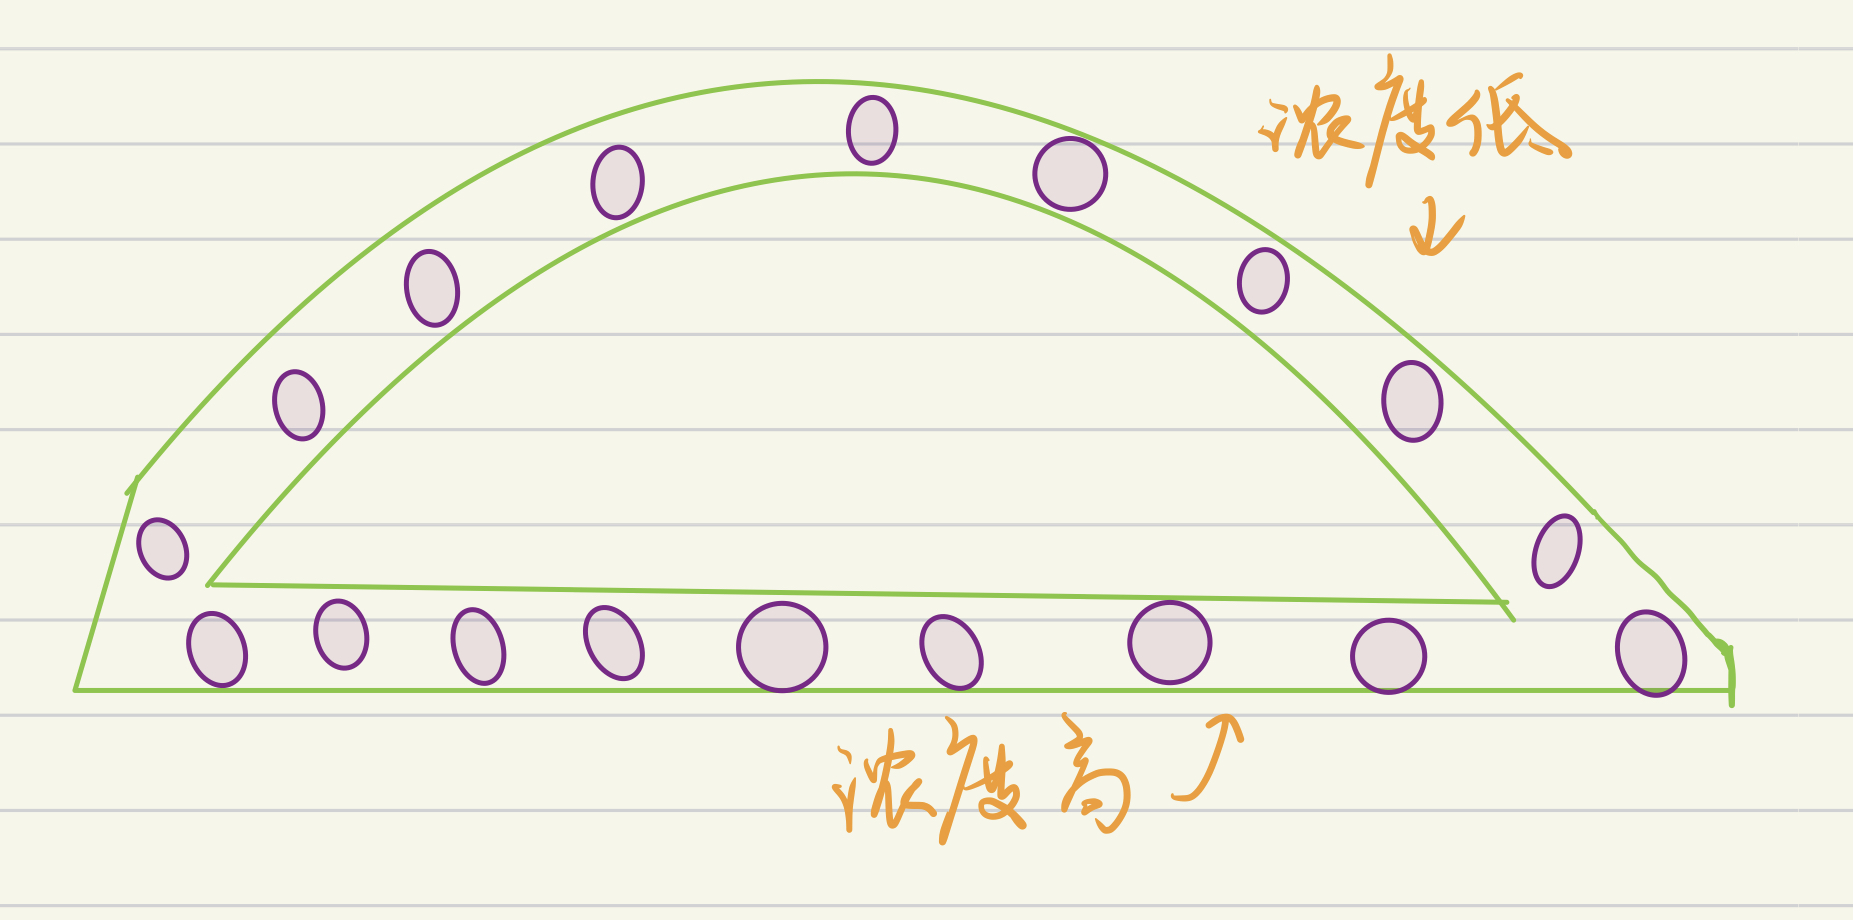
\includegraphics[width = 0.5\textwidth]{assets/ant.jpeg}
    \caption{\label{fig ant.jpeg}信息素示意图}
\end{figure}
图4-1可以帮助更好地理解蚁群(ant colony optimization,ACO)原理。假设蚂蚁走两条不一样长的路,可以留下的信息素是一样多的,那么越短的路信息素浓度越高,浓度与路径长度大致成反比。在之后的迭代,也就是第二轮蚂蚁寻路时,将会根据上一波蚂蚁的信息素来寻找路径,浓度高的路走的概率越高,第二轮结束时更新信息素。重复这样的迭代,直到最后,结果将趋近于最优路径。和模拟退火类似,我们约定一些计算方法来将此过程数学化。
\subsection{初始化}
在问题求解前,我们需要定义以下几个常量:蚂蚁数量m,总迭代次数T,挥发系数$\rho$,信息素因子$\alpha$,启发函数因子$\beta$,信息素常量Q,在后续将讲解每个常量的具体用处。

同时,我们定义信息素矩阵$A_{t}$来储存第t次寻路时的信息素$\tau(t)$,根据点的总数量n,$A_{t}$矩阵被定义为$n\times n$的矩阵。定义$\tau_{i j}(t)$为$A_{t}$的(i,j)项,表示第t次寻路时点i到j的信息素浓度,若是不可直达路径设置为0,初始化时可达的$\tau(0)$设置为常数C。

对于需要求解的问题,定义D矩阵,$d_{ij}$表示i点到j点的距离,不可达设置为$\infty$.

其中,m不宜过大,也不宜过小,若m过大会导致每条路径趋于平均,收敛速度更慢,m过小则可能出现未搜索但已被舍弃的道路,使算法过早地收敛。我们可以通过改变总迭代次数来使计算次数增加,结果更精确。
\subsection{状态转移方程}
蚁群算法的特点是微观与宏观相结合,微观指的是单个的蚂蚁,宏观指的是无数蚂蚁组成的蚁群,在每一只单个蚂蚁都遵循相同的行路准则这个基础上,蚁群便能实现单个蚂蚁无法实现的目标。在寻路问题的理解便是,每一个蚂蚁都会按照一定的算法来选择自己可移动的下一个点,计算每次的寻路过程,直到形成达到目标道路。
\subsubsection{微观状态转移:单个蚂蚁改变位置}
这里的状态转移是微观下的概念,指的是第k只蚂蚁从i点至j点遵循的概率计算方法,用$P_{i j}^k$表示。$(1\le k\le m)$

与一般的蚁群不同地,对每一只蚂蚁k动态定义集合$v_{i}^{k}$,记录此蚂蚁在i点处可以访问的点,若不可访问概率设置为0。$v_{i}^{k}$初始化为所有与i点连通的点,若蚂蚁在i点访问过某一点q,则在$v_{i}^{k}$中删去q点,即蚂蚁可以重复访问一点q,但不能重复从另一点i访问q。

此外,为了防止出现部分死路,从i点到j点,j的可访问集合不可为$\emptyset$.比如在示例图2-2的图中,蚂蚁从点1开始$v_{1}=\{2\}$,访问点2后更新$v_{1}=\emptyset$,$v_{2}=\{1,3,4,5\}$.此时由于点1对应空集,不可重新访问,从$v_{2}$中删去1.

令$\eta_{ij} =\frac{ \tau_{ij}^{\alpha}(t)}{d_{ij}^{\beta}}$.
\[P_{ij}^{k}=\begin{cases}
	\frac{\eta_{ij}}{\Sigma_{s\in v_{i}^{k}}\eta_{is}} & j \in v_{i}^{k}\\
	0 & j \notin v_{i}^{k}\\
\end{cases}
\]

对同一状态下给定的点i,分母是固定的。因此这个概率代表的是:信息素$\tau$越大,两点间距离越小,选择的概率越大。$\alpha$和 $\beta$分别表示两个值的重要程度,设置越大的数越重要,合理的取值会影响寻路的收敛范围和运算速度。通常取值在(0,4)之间即可,不超过5.

\subsubsection{宏观状态转移:更新信息素矩阵}
当前迭代次数为t,在所有蚂蚁寻路完成后,更新t+1的信息素矩阵,进入下轮迭代。信息素更新的计算方法满足:

$\tau_{ij}(t+1)=\tau_{ij}(t)(1-\rho)+\Delta \tau_{ij}$
其中$\Delta \tau_{ij}=\Sigma_{k=1}^{m}\Delta\tau_{ij}^{k}$,即新增的信息素为所有走过ij的蚂蚁信息素增量的和。关于$\Delta\tau_{ij}^{k}$的算法大致有三种模型,这里选用了最常用的蚁周模型,$\Delta\tau_{ij}^{k}=\frac{Q}{L_{k}}$,其中$L_{k}$是第k只蚂蚁本轮迭代走过的路径总长度,Q为常数,$\rho$为先前设置过的常数挥发系数,取值(0,1)。

对于另外两种信息素算法——蚁密、蚁量模型,侧重于局部的思想,在每次蚂蚁更新位置时完成信息素更新,分别是计算信息素增量为$\frac{Q}{d_{ij}}$和Q。蚁周模型侧重于全局的更新。
\subsection{具体步骤}
\begin{enumerate}
	\item 按照4.2节进行初始化。
	\item 随机布置蚂蚁的位置进行寻路。对每一只蚂蚁k,使用一个二维n阶数组V保存$v_{i}^{k}$,即其可以访问的点,按4.3.1的规则进行更新。
	\item 使用一个集合存储蚂蚁已访问的点,每走一步判断蚂蚁是否已访问过所有途径点集的点,如果已访问完毕结束本轮寻路。
	\item 更新信息素矩阵。
	\item 重复2,3,4,步直到迭代次数T次后结束。
\end{enumerate}
\newpage
\section{推广与其他}
\setcounter{figure}{0}
\subsection{实际推广:建立地铁站数据库}
为了将数量庞大的地铁站直观化为一张图,我尝试进行了简单的图数据库建立。
\subsubsection{整理数据}
从北京地铁官方网站上可以查询到北京地铁的多种数据。这里使用了地铁站各站点名称、站间距离这两项数据。

将其整理为csv文件:如图5-1。
\begin{figure}[h]
	\vspace{-5pt}
	\centering
	\subfloat[地铁站名]
	{
		\begin{minipage}{0.4\linewidth}
			\label{label.1}
			\centering
			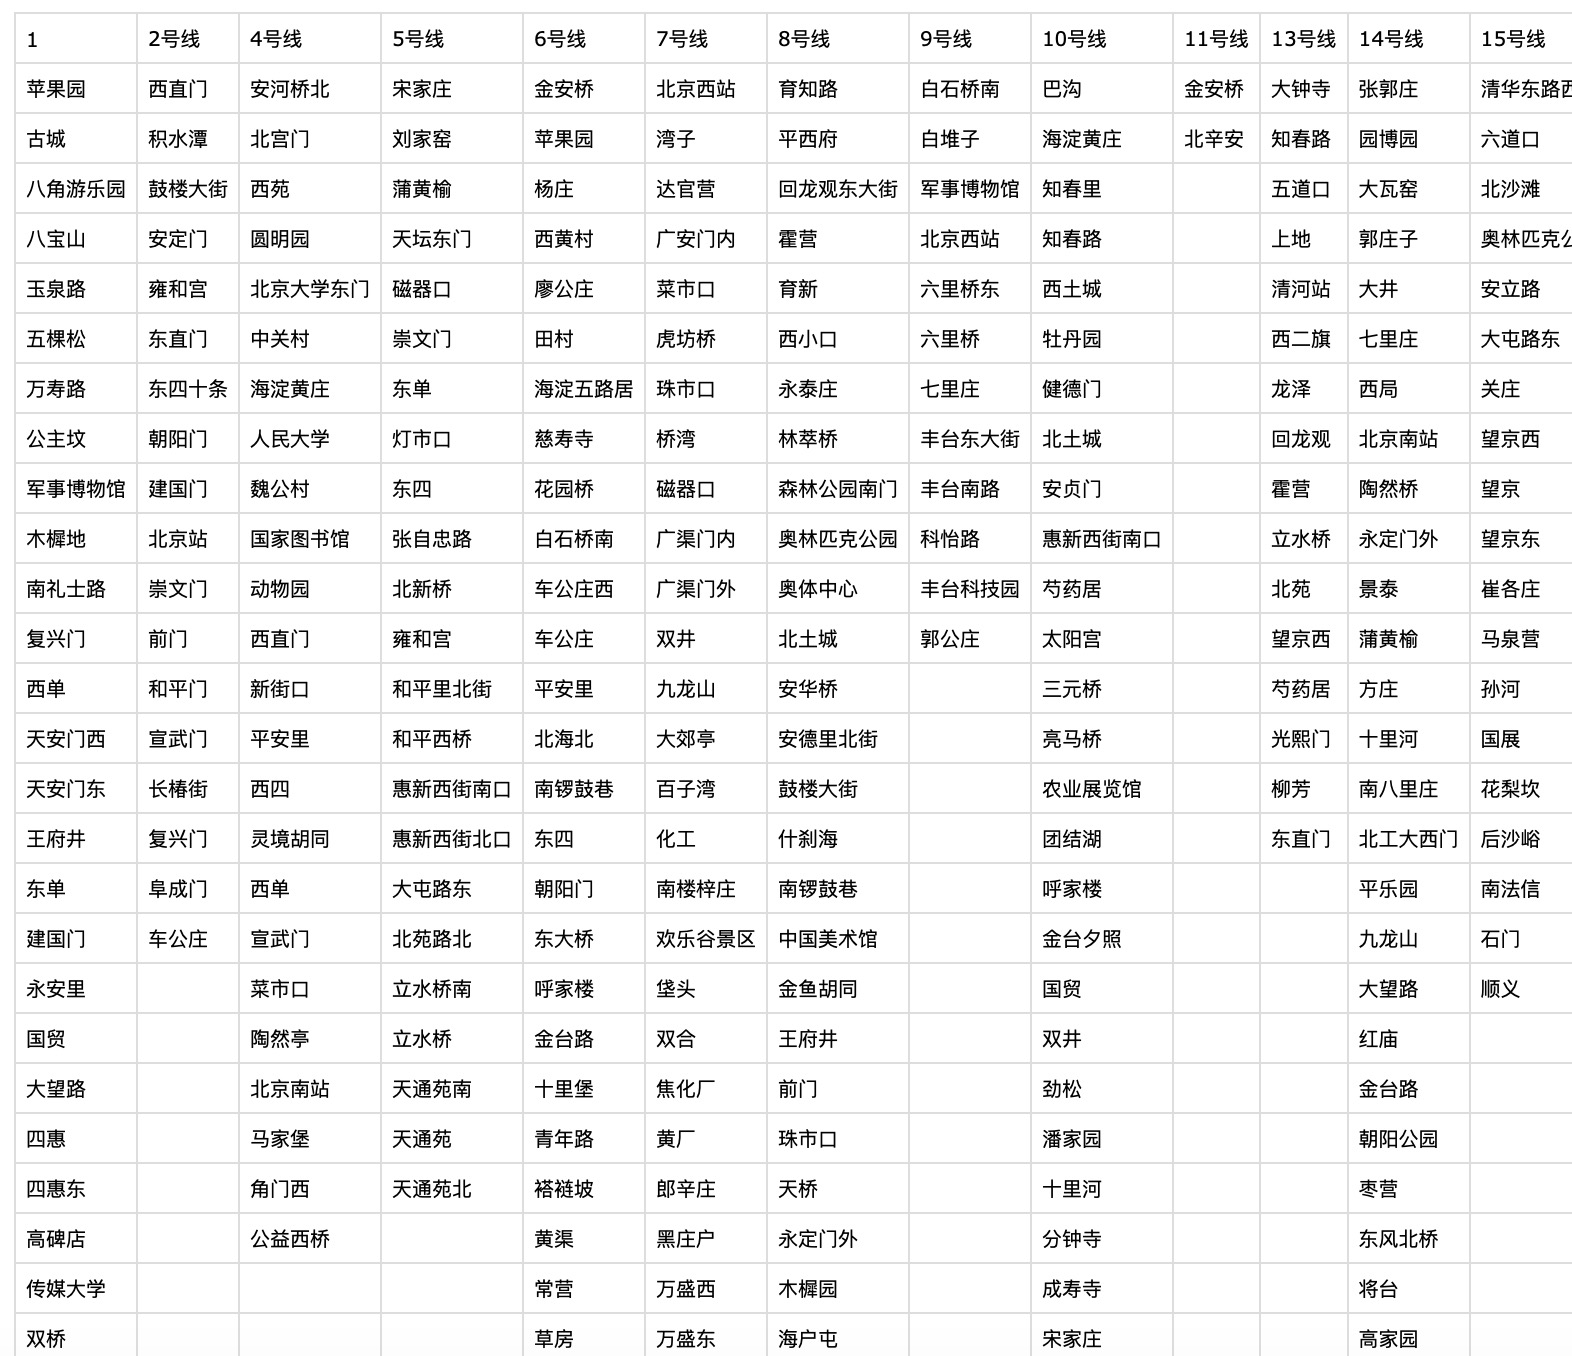
\includegraphics[width=1\textwidth]{assets/station.jpg}			
		\end{minipage}
	}
\hspace{10mm}
	\subfloat[站间距离]{
		\begin{minipage}{0.4\linewidth}
			\label{label.2}
			\centering
			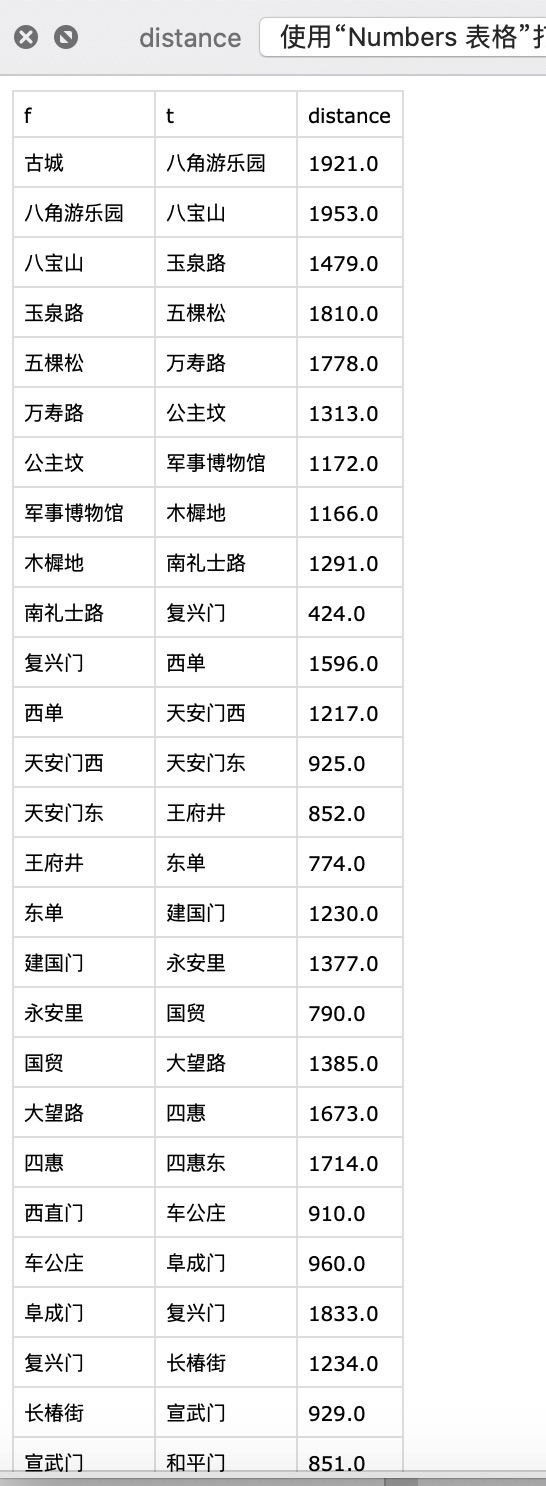
\includegraphics[width=0.5\textwidth]{assets/distance.jpg}	
		\end{minipage}
	}
	\caption{数据表格}
	\label{label}	
\end{figure}

\subsubsection{结合neo4j的地铁数据库}
\begin{enumerate}
\renewcommand{\labelenumi}{(\theenumi)}
\item 使用如下CQL语句添加点:
\begin{lstlisting}
LOAD CSV WITH HEADERS  FROM "file:///allstation.csv" AS line
CREATE(:station{name:line.name})
\end{lstlisting}
\item 在点之间添加关系,并记录距离distance的值
\begin{lstlisting}
LOAD CSV WITH HEADERS FROM "file:///distance.csv" AS line
match (from:station{name:line.f}),(to:station{name:line.t})
merge (from)-[r: to {distance:line.distance}]->(to);
\end{lstlisting}
\item 通过结合使用neo4j及neo2py提供的api接口,我们可以方便直观地查询地铁站的多种信息,并使用唯一数字编号的id以及distance值快速地将地铁信息转化为加权图。
\end{enumerate}
\begin{figure}[h]
    \centering
    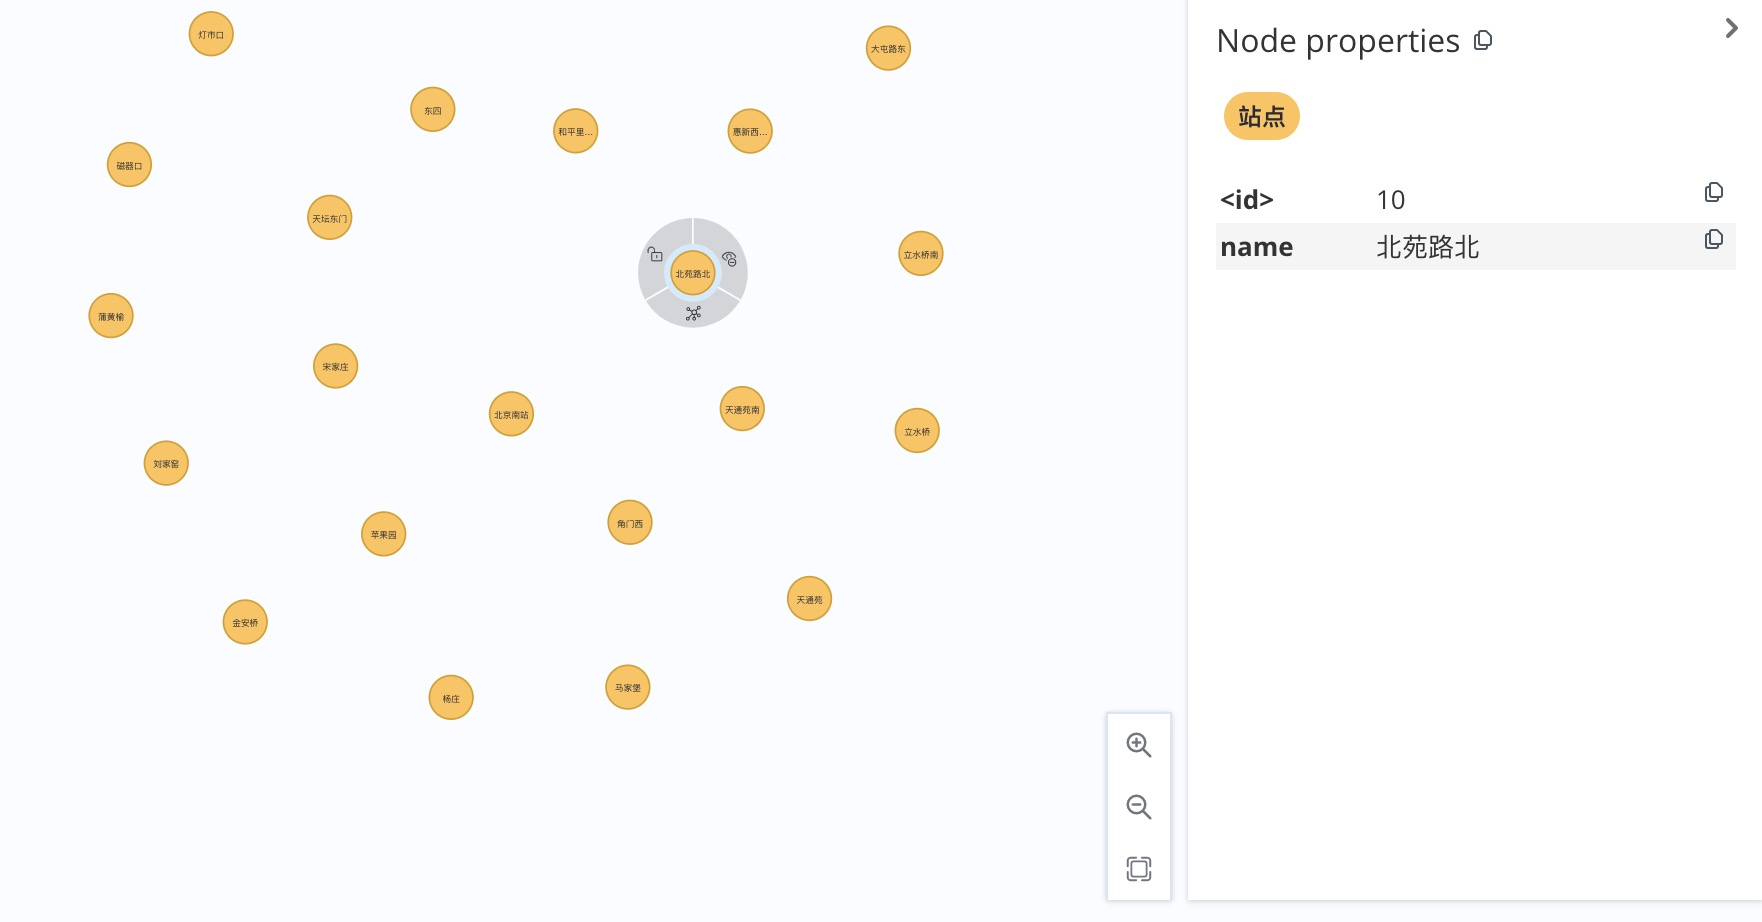
\includegraphics[width = 0.6\textwidth]{assets/neo4j-nodes.jpg}
    \caption{\label{fig neo4j-nodes.jpg}在neo4j中添加点}
\end{figure}
\begin{figure}[h]
    \centering
    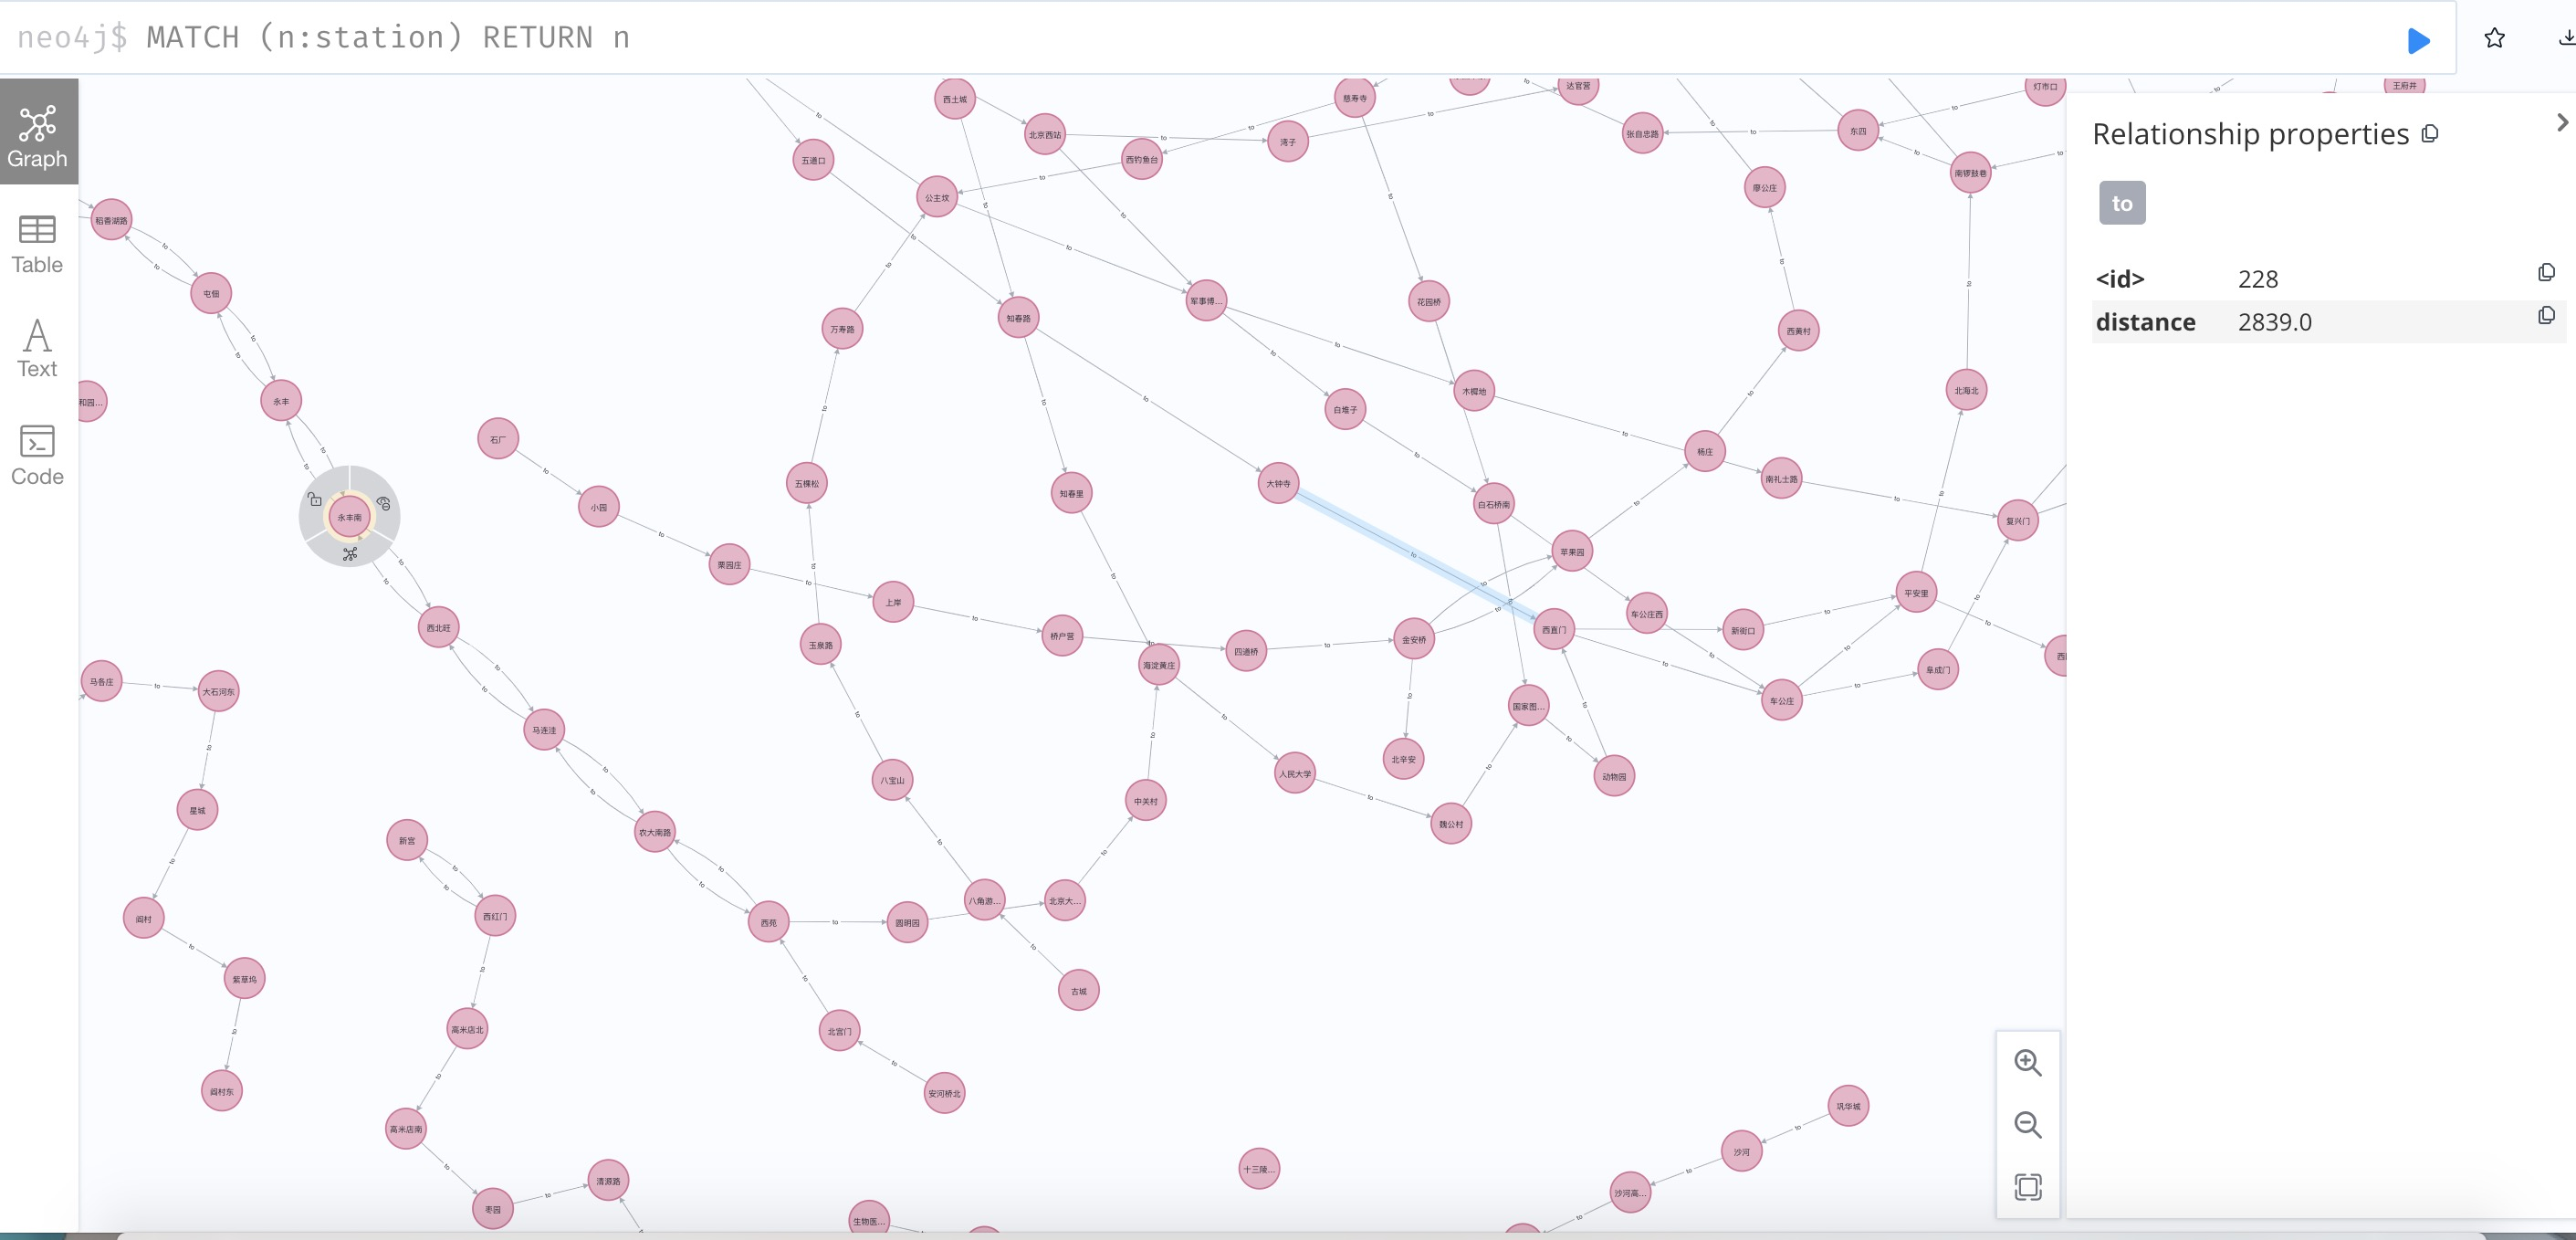
\includegraphics[width = 0.8\textwidth]{assets/neo4j-relationship.jpg}
    \caption{\label{fig neo4j-relationship.jpg}添加关系}
\end{figure}
~\
\subsection{其他思路}
在搜索资料的过程中,我发现本文的问题有点类似于2016年华为算法精英赛的题目,题目的说明更加详细,由于正文篇幅有限,原题贴在了附录上。(但不同的是原题有不成环的要求,而我自拟的题目假设里没有这个必要需求)

在思考我的问题时也参考了当时网上一些参赛选手的思路,发现对于优化和更好的解法,能学习的空间还非常大。有很多的更好的思路和优化方法,因为时间有限没有深挖,只是草草地浏览了解了一下,有点可惜。我在GitHub上找到了比赛冠军的源码和程序思路,源码有几千行,想自己完全重写复现不太可行……在此就简单地整理一下思路:
\begin{enumerate}
	\item 规模压缩,使用SPFA算法求出所有必经点之间的最短路径并记录(与我的Floyd方法类似,但在本例中性能更优,与Dijkstra heap差不多)
	\item 转化为atsp问题,即非对称tsp问题,可以理解为存在点i点j,i到j的距离与j到i是不一样的tsp问题。
	\item 使用LKH算法求解atsp问题。
	\item 根据所得路径检查有无重复使用的非必经点,若有,将这些点改为必经点,转到1重新求解,没有则求解成功。
\end{enumerate}
\subsection{LKH算法}
LKH算法或许是现在公认的最好的tsp问题解法,基于k-opt的思想,通过将图中的连接边切断、重连的方式一次次改进获得更好的路径解。

以下截自冠军队伍的程序思路,直观讲解了怎么理解k-opt。
\begin{figure}[h]
    \centering
    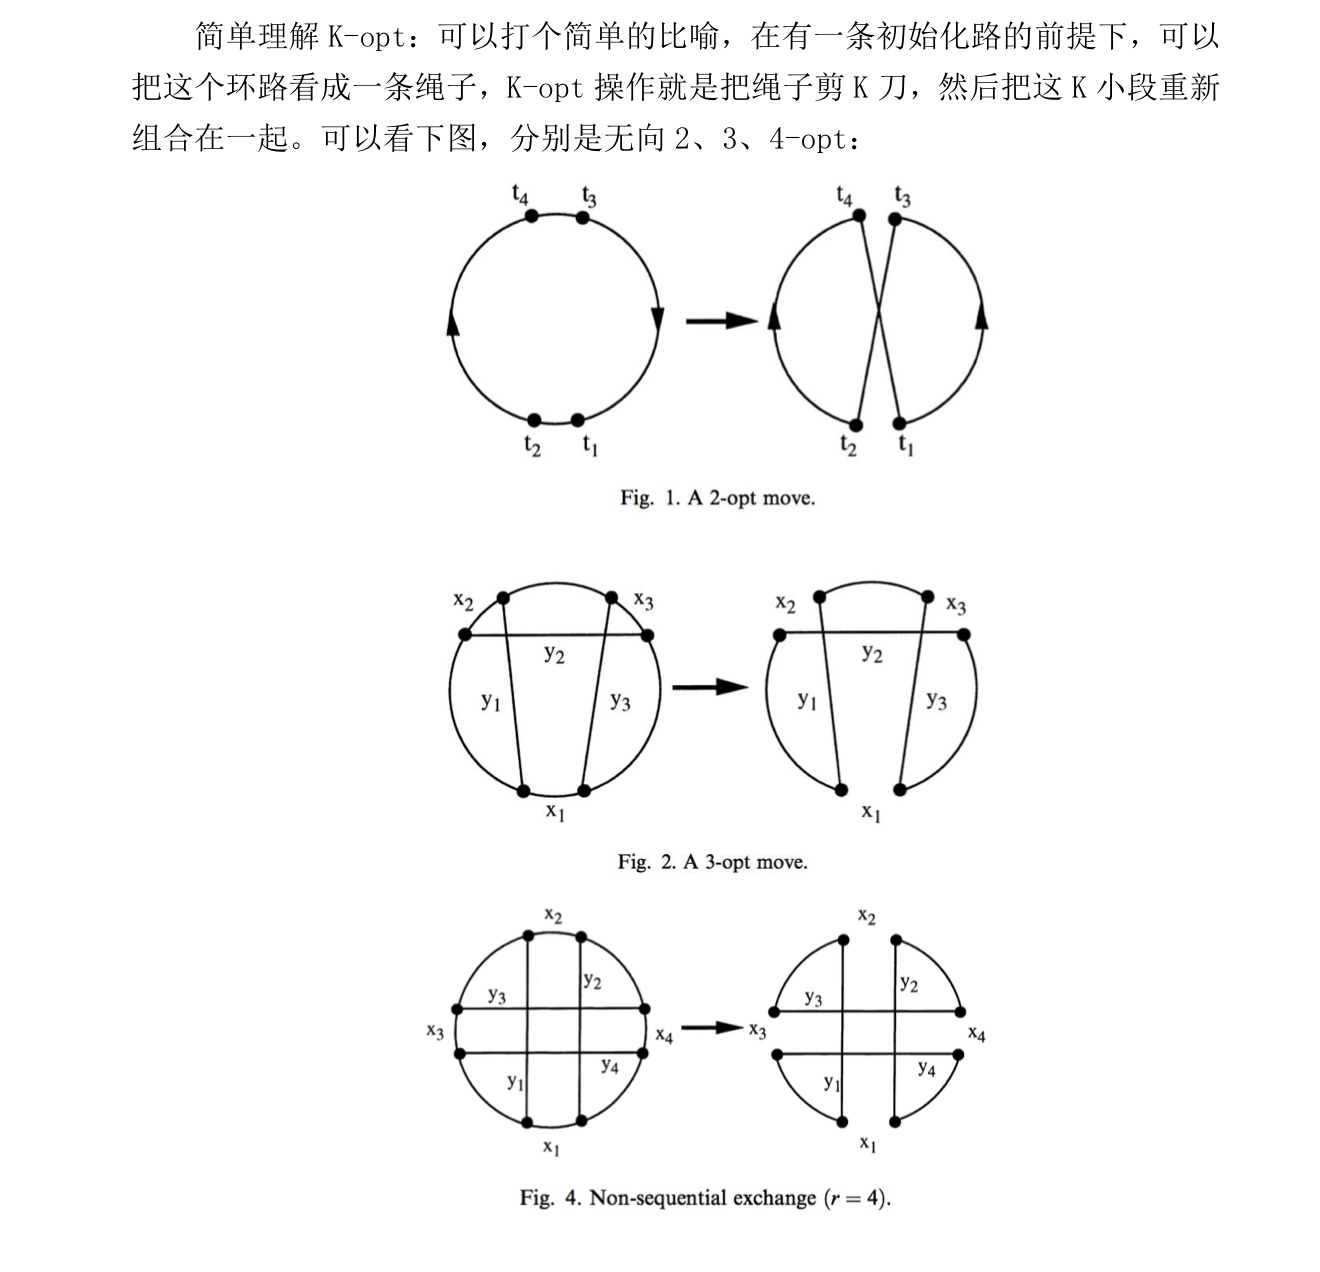
\includegraphics[width = 0.8\textwidth]{assets/kopt.jpg}
    \caption{\label{fig kopt.jpg}k-opt}
\end{figure}
其实opt就是交换的意思,我们在一个可行初始解的基础上交换k条边,若所得解更小则更优。比如在上图的2-opt中,选择两条不相邻的边(t1,t2),(t3,t4),交换所得的解就是(t1,t4),(t3,t2),或者(t1,t3),(t4,t2),在有向图中解更多。k-opt的时间复杂度为$O(n^k)$.

LKH算法通过实验测得一般的tsp问题在5-opt以内即可解决。主要思想就是在一个初始可行解中从起点1开始先交换两条边,若能得到更优解更新初始解,若不行交换三条边,直到交换五条边。若仍没有更优解,更换起点重新寻找。

k-opt有Sequential的要求,即顺序性。定义为:若删除的边集为$X=\{x_{i}\}$,增加的边集为$Y=\{y_{i} \}$,则有
\begin{enumerate}
	\item $x_{i}$与$y_{i}$有共同的端点,$y_{i}$与$x_{i+1}$也有共同的端点.
	\item XY没有公共边
	\item X总长度小于Y
	\item 交换后仍为可行解
\end{enumerate}
在图5-4中,示例的3-opt是Sequential的,而4-opt不是。

关于LKH算法涉及的内容很多,包括次梯度优化,最小生成树1-tree理论,a-nearness理论等等,此处只是简单地进行了介绍,此外LKH虽然是上个世纪提出的算法,但至今仍在不断更新,最新版的LKH-3可以解决的优化问题非常多。更详细的可以参阅参考文献中的lkh算法官网和其中的report的pdf文件,写得非常详细,此处不再赘述。
\subsection{总结}
这里干脆写一点自己对整个项目想说的话,关于这个问题刚接触时我是非常感兴趣的,最开始是很想知道北京地铁走完所有站点最短的路径,所以才试着挑战自己一个人来完成这个题目。不过结果是我对选择的方法还是不太满意,因为这个问题还没有一个统一的解法,所以尝试了很多思路比较可行性,也深深感觉到受限于学识,只实现了最简单的方法,没有什么新意。但这个过程中我发现了还有很多值得去学习的东西,虽然自己现在还没有时间深入地去理解他们,不过也算是敲开了优化这个学科的大门,知道了原来还有这么多理论方法,感觉自己可以学习的非常非常多。

这一节和上一节都是我在现有的思想上,加上了一点点的自己的思路尝试。本来没来得及写出完整的程序是不想写上来的,可能写出来的东西错误很多,但接下来的一段时间应该不会再接触这个项目了……所以还是记录了下来,说不定以后有时间就写出来东西了呢。还有这个简单提了一下的地铁站数据库,最后没做完是因为数据好像有点问题,在从官网上复制下来的时候缺了一些站点,但又没有那个耐心去一个个校对……

可能我呈现出来的结果比较不尽人意,甚至忙活了半天也没有解决最早提出的那个地铁问题,自己也没有什么信心。不过在作业的推动下也算是学到了不少东西,激发了一些学习的兴趣,还是很感谢能有这样的机会。我也是很想继续研究这个问题的,希望以后能有机会在这个基础上,做出来我更满意的东西。
\newpage
\addcontentsline{toc}{section}{附录}
\section*{附录}
\setcounter{footnote}{0}
\setcounter{section}{0}
\section{源码}
\subsection{使用networkx绘制图}
\lstinputlisting[language = Python]{src/drawnet.py}
\subsection{深搜}
\lstinputlisting[language = Python]{src/Search.py}
\subsection{模拟退火}
部分参考、引用了参考文献[6],[7]
\lstinputlisting[language = Python]{src/SA.py}
\subsection{Floyd算法}
\lstinputlisting[language = Python]{src/floyd.py}
\section{部分结果}
\subsection{2-1示例图}
初始: [[0, 6, 8, 1, inf, inf, inf, inf, inf, inf, inf],
 [6, 0, inf, 2, 1, inf, inf, inf, inf, inf, inf],
 [8, inf, 0, 5, 5, 1, 2, inf, inf, inf, inf],
 [1, 2, 5, 0, inf, inf, 6, inf, inf, inf, 2],
 [inf, 1, 5, inf, 0, 3, inf, 2, 9, inf, inf],
 [inf, inf, 1, inf, 3, 0, 4, inf, 6, inf, inf],
 [inf, inf, 2, 6, inf, 4, 0, inf, 3, 1, inf],
 [inf, inf, inf, inf, 2, inf, inf, 0, 7, inf, 9],
 [inf, inf, inf, inf, 9, 6, 3, 7, 0, 1, 2],
 [inf, inf, inf, inf, inf, inf, 1, inf, 1, 0, 4],
 [inf, inf, inf, 2, inf, inf, inf, 9, 2, 4, 0]]
 
 
 结果:[[0, 3, 6, 1, 4, 7, 7, 6, 5, 6, 3],
 [3, 0, 5, 2, 1, 4, 7, 3, 6, 7, 4],
 [6, 5, 0, 5, 4, 1, 2, 6, 4, 3, 6],
 [1, 2, 5, 0, 3, 6, 6, 5, 4, 5, 2],
 [4, 1, 4, 3, 0, 3, 6, 2, 7, 7, 5],
 [7, 4, 1, 6, 3, 0, 3, 5, 5, 4, 7],
 [7, 7, 2, 6, 6, 3, 0, 8, 2, 1, 4],
 [6, 3, 6, 5, 2, 5, 8, 0, 7, 8, 7],
 [5, 6, 4, 4, 7, 5, 2, 7, 0, 1, 2],
 [6, 7, 3, 5, 7, 4, 1, 8, 1, 0, 3],
 [3, 4, 6, 2, 5, 7, 4, 7, 2, 3, 0]]
 
最短路径走法: [[[1],[1, 4, 2],[1, 4, 3], [1, 4], [1, 4, 2, 5], [1, 4, 2, 5, 6], [1, 4, 7], [1, 4, 2, 5, 8], [1, 4, 11, 9], [1, 4, 11, 9, 10], [1, 4, 11]], [[2, 4, 1], [2], [2, 5, 6, 3], [2, 4], [2, 5], [2, 5, 6], [2, 5, 6, 3, 7], [2, 5, 8], [2, 4, 11, 9], [2, 4, 11, 9, 10], [2, 4, 11]], [[3, 4, 1], [3, 6, 5, 2], [3], [3, 4], [3, 6, 5], [3, 6], [3, 7], [3, 6, 5, 8], [3, 7, 10, 9], [3, 7, 10], [3, 7, 10, 9, 11]], [[4, 1], [4, 2], [4, 3], [4], [4, 2, 5], [4, 2, 5, 6], [4, 7], [4, 2, 5, 8], [4, 11, 9], [4, 11, 9, 10], [4, 11]], [[5, 2, 4, 1], [5, 2], [5, 6, 3], [5, 2, 4], [5], [5, 6], [5, 6, 3, 7], [5, 8], [5, 2, 4, 11, 9], [5, 6, 3, 7, 10], [5, 2, 4, 11]], [[6, 3, 4, 1], [6, 5, 2], [6, 3], [6, 3, 4], [6, 5], [6], [6, 3, 7], [6, 5, 8], [6, 3, 7, 10, 9], [6, 3, 7, 10], [6, 3, 7, 10, 9, 11]], [[7, 4, 1], [7, 3, 6, 5, 2], [7, 3], [7, 4], [7, 3, 6, 5], [7, 3, 6], [7], [7, 3, 6, 5, 8], [7, 10, 9], [7, 10], [7, 10, 9, 11]], [[8, 5, 2, 4, 1], [8, 5, 2], [8, 5, 6, 3], [8, 5, 2, 4], [8, 5], [8, 5, 6], [8, 5, 6, 3, 7], [8], [8, 9], [8, 9, 10], [8, 5, 2, 4, 11]], [[9, 11, 4, 1], [9, 11, 4, 2], [9, 10, 7, 3], [9, 11, 4], [9, 11, 4, 2, 5], [9, 10, 7, 3, 6], [9, 10, 7], [9, 8], [9], [9, 10], [9, 11]], [[10, 9, 11, 4, 1], [10, 9, 11, 4, 2], [10, 7, 3], [10, 9, 11, 4], [10, 7, 3, 6, 5], [10, 7, 3, 6], [10, 7], [10, 9, 8], [10, 9], [10], [10, 9, 11]], [[11, 4, 1], [11, 4, 2], [11, 9, 10, 7, 3], [11, 4], [11, 4, 2, 5], [11, 9, 10, 7, 3, 6], [11, 9, 10, 7], [11, 4, 2, 5, 8], [11, 9], [11, 9, 10],[11]]]

过所有点且权和小于等于20的解:(1, 4, 2, 5, 8, 5, 6, 3, 6, 3, 7, 10, 9, 11), (1, 4, 2, 5, 8, 5, 6, 3, 7, 10, 9, 11), (2, 5, 8, 5, 6, 3, 7, 10, 7, 10, 9, 11, 4, 1), (3, 6, 3, 7, 10, 9, 10, 9, 11, 4, 1, 4, 2, 5, 8), (3, 6, 3, 7, 10, 9, 11, 4, 1, 4, 2, 5, 2, 5, 8), (3, 6, 3, 7, 10, 9, 11, 4, 1, 4, 2, 5, 8), (3, 6, 3, 7, 10, 9, 11, 4, 1, 4, 2, 5, 8, 5), (3, 6, 3, 7, 10, 9, 11, 4, 1, 4, 2, 5, 8, 5, 2), (3, 6, 5, 8, 5, 2, 4, 1, 4, 11, 9, 10, 7), (3, 6, 5, 8, 5, 2, 4, 1, 4, 11, 9, 10, 7, 10), (6, 3, 6, 5, 8, 5, 2, 4, 1, 4, 11, 9, 10, 7), (6, 3, 7, 10, 7, 10, 9, 11, 4, 1, 4, 2, 5, 2, 5, 8), (6, 3, 7, 10, 7, 10, 9, 11, 4, 1, 4, 2, 5, 8), (6, 3, 7, 10, 7, 10, 9, 11, 4, 1, 4, 2, 5, 8, 5), (6, 3, 7, 10, 9, 10, 9, 11, 4, 1, 4, 2, 5, 2, 5, 8), (6, 3, 7, 10, 9, 10, 9, 11, 4, 1, 4, 2, 5, 8), (6, 3, 7, 10, 9, 10, 9, 11, 4, 1, 4, 2, 5, 8, 5), (6, 3, 7, 10, 9, 11, 4, 1, 4, 2, 4, 2, 5, 8), (6, 3, 7, 10, 9, 11, 4, 1, 4, 2, 5, 2, 5, 8), (6, 3, 7, 10, 9, 11, 4, 1, 4, 2, 5, 8), (6, 3, 7, 10, 9, 11, 4, 1, 4, 2, 5, 8, 5), (6, 3, 7, 10, 9, 11, 4, 1, 4, 2, 5, 8, 5, 2), (6, 3, 7, 10, 9, 11, 4, 2, 4, 1, 4, 2, 5, 8), (6, 3, 7, 10, 9, 11, 4, 2, 5, 8, 5, 2, 4, 1), (7, 3, 6, 3, 7, 10, 9, 11, 4, 1, 4, 2, 5, 8), (8, 5, 2, 5, 6, 3, 7, 10, 7, 10, 9, 11, 4, 1), (9, 10, 7, 3, 6, 5, 8, 5, 2, 4, 11, 4, 1), (10, 7, 3, 6, 3, 7, 10, 9, 11, 4, 1, 4, 2, 5, 8), (11, 9, 10, 7, 3, 6, 5, 8, 5, 2, 4, 1), (11, 9, 10, 7, 3, 6, 5, 8, 5, 2, 4, 1, 4), (11, 9, 10, 9, 10, 7, 3, 6, 5, 8, 5, 2, 4, 1)
\section{运行环境}
若无另外说明,本文所有运行环境为python3.8,anaconda3,macOS Catalina10.15.16,neo4j-community-4.4.12.
\section{2016华为挑战赛题目}
前言

赛题源自“未来网络”业务发放中的路由计算问题。算路问题属于基础算法问题,在图论、网络、交通等各个方面均有着广泛的研究与运用,里面不乏一些经典的算法,例如最短路中的广度优先搜索,Dijkstra算法等。网络算路问题的更优算法实现对于网络资源高效配置具有重要价值。

初赛赛题:

给定一个带权重的有向图G=(V,E),V为顶点集,E为有向边集,每一条有向边均有一个权重。对于给定的顶点s、t,以及V的子集V',寻找从s到t的不成环有向路径P,使得P经过V'中所有的顶点(对经过V'中节点的顺序不做要求)。

若不存在这样的有向路径P,则输出无解,程序运行时间越短,则视为结果越优;若存在这样的有向路径P,则输出所得到的路径,路径的权重越小,则视为结果越优,在输出路径权重一样的前提下,程序运行时间越短,则视为结果越优。

说明:
\begin{enumerate}
	\item 图中所有权重均为[1,20]内的整数;
	\item 任一有向边的起点不等于终点;
	\item 连接顶点A至顶点B的有向边可能超过一条,其权重可能一样,也可能不一样;
	\item 该有向图的顶点不会超过600个,每个顶点出度(以该点为起点的有向边的数量)不超过8;
	\item V'中元素个数不超过50;
	\item 从s到t的不成环有向路径P是指,P为由一系列有向边组成的从s至t的有向连通路径,且不允许重复经过任一节点;
	\item 路径的权重是指所有组成该路径的所有有向边的权重之和。
\end{enumerate}
复赛赛题:

给定一个带权重的有向图G=(V,E),V为顶点集,E为有向边集,每一条有向边均有一个权重。对于给定的顶点s、t,以及V的子集V’和V’’,寻找从s到t的两条不成环的有向路径P’和P’’,使得P’经过V’中所有的顶点,而P’’经过V’’中所有的顶点(对P’经过V’中顶点的顺序以及P’’经过V’’中顶点的顺序不做要求)。

若不同时存在这样的两条有向路径,则输出无解,程序运行时间越短,则视为结果越优; 若同时存在这样的两条有向路径,则输出得到的两条路径,按下列优先级从高到低评价结果优劣:
\begin{enumerate}
	\item 路径P’和P’’重合的有向边个数越少,则视为结果越优;
	\item  在两条路径重合的有向边个数一样的情况下,两条路径权重总和越少,则视为结果越优;
	\item 在上述两个指标一样的情况下,程序运行时间越短,则视为结果越优。
\end{enumerate}
说明:
\begin{enumerate}
	\item 图中所有权重均为[1,100]内的整数;
	\item 任一有向边的起点不等于终点;
	\item 连接顶点A至顶点B的有向边可能超过一条,其权重可能一样,也可能不一样;
	\item 该有向图的顶点不会超过2000个,每个顶点出度(以该点为起点的有向边的数量)不超过20;
	\item V’和V’’中元素个数均不超过100,交集为空,且不包含起始顶点s和终止顶点t;
	\item 从s到t的不成环有向路径P是指,P为由一系列有向边组成的从s至t的有向连通路径,且不允许重复经过任一顶点;
	\item 路径的权重是指所有组成该路径的所有有向边的权重之和(重复边的权重应分别在两条路径中各计算一次)。
\end{enumerate}
网上应该还有决赛赛题和数据集可以参考。
\addcontentsline{toc}{section}{参考文献}
\begin{thebibliography}{1}
\bibitem{wang}王艳愉,李强.必经点约束型最短路径问题的研究[J].微型机与应用,2017,(22):26-29.
\bibitem{d}刁在筠,刘桂真.运筹学第四版[M].北京:高等教育出版社,2016.
\bibitem{h}胡云权.运筹学教程[M].北京:清华大学出版社,2018.
\bibitem{bj}\href{https://www.bjsubway.com/}{北京市地铁运营有限公司.北京地铁}[DB/OL].bjsubway,2022.\footnote{以下在线资料都插入了网址超链接,可直接点击名称访问}
\bibitem{a}\href{https://www.flyai.com/article/artfd2570e423665ccbf7f9929c?type=e}{flyai.Python数模笔记-NetworkX 最短路径}[EB/OL].flyai,2021.
\bibitem{t}\href{https://github.com/kellenf/TSP\_collection}{kellenf.TSP算法全复现}[EB/OL].github,2020.
\bibitem{t}\href{https://blog.csdn.net/weixin\_37522117/article/details/125149593?spm=1001.2101.3001.6650.3&utm\_medium=distribute.pc\_relevant.none-task-blog-2\%7Edefault\%7EESLANDING\%7Edefault-3-125149593-blog-109305769.pc\_relevant\_landingrelevant&depth\_1-utm\_source=distribute.pc\_relevant.none-task-blog-2\%7Edefault\%7EESLANDING\%7Edefault-3-125149593-blog-109305769.pc\_relevant\_landingrelevant}{模拟退火算法求解TSP问题(python)}[EB/OL].csdn,2022.
\bibitem{lkh}\href{http://comopt.ifi.uni-heidelberg.de/software/TSPLIB95/}{TSPLIB 标准数据集},\href{http://comopt.ifi.uni-heidelberg.de/software/TSPLIB95/STSP.html}{Solutions}[DB/OL],2007
\bibitem{lkh3}\href{http://webhotel4.ruc.dk/~keld/research/LKH-3/}{LKH-3官网}[EB/OL],2022.
\end{thebibliography}
\end{document}